% Options for packages loaded elsewhere
% Options for packages loaded elsewhere
\PassOptionsToPackage{unicode}{hyperref}
\PassOptionsToPackage{hyphens}{url}
\PassOptionsToPackage{dvipsnames,svgnames,x11names}{xcolor}
%
\documentclass[
  letterpaper,
  DIV=11,
  numbers=noendperiod]{scrartcl}
\usepackage{xcolor}
\usepackage{amsmath,amssymb}
\setcounter{secnumdepth}{-\maxdimen} % remove section numbering
\usepackage{iftex}
\ifPDFTeX
  \usepackage[T1]{fontenc}
  \usepackage[utf8]{inputenc}
  \usepackage{textcomp} % provide euro and other symbols
\else % if luatex or xetex
  \usepackage{unicode-math} % this also loads fontspec
  \defaultfontfeatures{Scale=MatchLowercase}
  \defaultfontfeatures[\rmfamily]{Ligatures=TeX,Scale=1}
\fi
\usepackage{lmodern}
\ifPDFTeX\else
  % xetex/luatex font selection
\fi
% Use upquote if available, for straight quotes in verbatim environments
\IfFileExists{upquote.sty}{\usepackage{upquote}}{}
\IfFileExists{microtype.sty}{% use microtype if available
  \usepackage[]{microtype}
  \UseMicrotypeSet[protrusion]{basicmath} % disable protrusion for tt fonts
}{}
\makeatletter
\@ifundefined{KOMAClassName}{% if non-KOMA class
  \IfFileExists{parskip.sty}{%
    \usepackage{parskip}
  }{% else
    \setlength{\parindent}{0pt}
    \setlength{\parskip}{6pt plus 2pt minus 1pt}}
}{% if KOMA class
  \KOMAoptions{parskip=half}}
\makeatother
% Make \paragraph and \subparagraph free-standing
\makeatletter
\ifx\paragraph\undefined\else
  \let\oldparagraph\paragraph
  \renewcommand{\paragraph}{
    \@ifstar
      \xxxParagraphStar
      \xxxParagraphNoStar
  }
  \newcommand{\xxxParagraphStar}[1]{\oldparagraph*{#1}\mbox{}}
  \newcommand{\xxxParagraphNoStar}[1]{\oldparagraph{#1}\mbox{}}
\fi
\ifx\subparagraph\undefined\else
  \let\oldsubparagraph\subparagraph
  \renewcommand{\subparagraph}{
    \@ifstar
      \xxxSubParagraphStar
      \xxxSubParagraphNoStar
  }
  \newcommand{\xxxSubParagraphStar}[1]{\oldsubparagraph*{#1}\mbox{}}
  \newcommand{\xxxSubParagraphNoStar}[1]{\oldsubparagraph{#1}\mbox{}}
\fi
\makeatother

\usepackage{color}
\usepackage{fancyvrb}
\newcommand{\VerbBar}{|}
\newcommand{\VERB}{\Verb[commandchars=\\\{\}]}
\DefineVerbatimEnvironment{Highlighting}{Verbatim}{commandchars=\\\{\}}
% Add ',fontsize=\small' for more characters per line
\usepackage{framed}
\definecolor{shadecolor}{RGB}{241,243,245}
\newenvironment{Shaded}{\begin{snugshade}}{\end{snugshade}}
\newcommand{\AlertTok}[1]{\textcolor[rgb]{0.68,0.00,0.00}{#1}}
\newcommand{\AnnotationTok}[1]{\textcolor[rgb]{0.37,0.37,0.37}{#1}}
\newcommand{\AttributeTok}[1]{\textcolor[rgb]{0.40,0.45,0.13}{#1}}
\newcommand{\BaseNTok}[1]{\textcolor[rgb]{0.68,0.00,0.00}{#1}}
\newcommand{\BuiltInTok}[1]{\textcolor[rgb]{0.00,0.23,0.31}{#1}}
\newcommand{\CharTok}[1]{\textcolor[rgb]{0.13,0.47,0.30}{#1}}
\newcommand{\CommentTok}[1]{\textcolor[rgb]{0.37,0.37,0.37}{#1}}
\newcommand{\CommentVarTok}[1]{\textcolor[rgb]{0.37,0.37,0.37}{\textit{#1}}}
\newcommand{\ConstantTok}[1]{\textcolor[rgb]{0.56,0.35,0.01}{#1}}
\newcommand{\ControlFlowTok}[1]{\textcolor[rgb]{0.00,0.23,0.31}{\textbf{#1}}}
\newcommand{\DataTypeTok}[1]{\textcolor[rgb]{0.68,0.00,0.00}{#1}}
\newcommand{\DecValTok}[1]{\textcolor[rgb]{0.68,0.00,0.00}{#1}}
\newcommand{\DocumentationTok}[1]{\textcolor[rgb]{0.37,0.37,0.37}{\textit{#1}}}
\newcommand{\ErrorTok}[1]{\textcolor[rgb]{0.68,0.00,0.00}{#1}}
\newcommand{\ExtensionTok}[1]{\textcolor[rgb]{0.00,0.23,0.31}{#1}}
\newcommand{\FloatTok}[1]{\textcolor[rgb]{0.68,0.00,0.00}{#1}}
\newcommand{\FunctionTok}[1]{\textcolor[rgb]{0.28,0.35,0.67}{#1}}
\newcommand{\ImportTok}[1]{\textcolor[rgb]{0.00,0.46,0.62}{#1}}
\newcommand{\InformationTok}[1]{\textcolor[rgb]{0.37,0.37,0.37}{#1}}
\newcommand{\KeywordTok}[1]{\textcolor[rgb]{0.00,0.23,0.31}{\textbf{#1}}}
\newcommand{\NormalTok}[1]{\textcolor[rgb]{0.00,0.23,0.31}{#1}}
\newcommand{\OperatorTok}[1]{\textcolor[rgb]{0.37,0.37,0.37}{#1}}
\newcommand{\OtherTok}[1]{\textcolor[rgb]{0.00,0.23,0.31}{#1}}
\newcommand{\PreprocessorTok}[1]{\textcolor[rgb]{0.68,0.00,0.00}{#1}}
\newcommand{\RegionMarkerTok}[1]{\textcolor[rgb]{0.00,0.23,0.31}{#1}}
\newcommand{\SpecialCharTok}[1]{\textcolor[rgb]{0.37,0.37,0.37}{#1}}
\newcommand{\SpecialStringTok}[1]{\textcolor[rgb]{0.13,0.47,0.30}{#1}}
\newcommand{\StringTok}[1]{\textcolor[rgb]{0.13,0.47,0.30}{#1}}
\newcommand{\VariableTok}[1]{\textcolor[rgb]{0.07,0.07,0.07}{#1}}
\newcommand{\VerbatimStringTok}[1]{\textcolor[rgb]{0.13,0.47,0.30}{#1}}
\newcommand{\WarningTok}[1]{\textcolor[rgb]{0.37,0.37,0.37}{\textit{#1}}}

\usepackage{longtable,booktabs,array}
\usepackage{calc} % for calculating minipage widths
% Correct order of tables after \paragraph or \subparagraph
\usepackage{etoolbox}
\makeatletter
\patchcmd\longtable{\par}{\if@noskipsec\mbox{}\fi\par}{}{}
\makeatother
% Allow footnotes in longtable head/foot
\IfFileExists{footnotehyper.sty}{\usepackage{footnotehyper}}{\usepackage{footnote}}
\makesavenoteenv{longtable}
\usepackage{graphicx}
\makeatletter
\newsavebox\pandoc@box
\newcommand*\pandocbounded[1]{% scales image to fit in text height/width
  \sbox\pandoc@box{#1}%
  \Gscale@div\@tempa{\textheight}{\dimexpr\ht\pandoc@box+\dp\pandoc@box\relax}%
  \Gscale@div\@tempb{\linewidth}{\wd\pandoc@box}%
  \ifdim\@tempb\p@<\@tempa\p@\let\@tempa\@tempb\fi% select the smaller of both
  \ifdim\@tempa\p@<\p@\scalebox{\@tempa}{\usebox\pandoc@box}%
  \else\usebox{\pandoc@box}%
  \fi%
}
% Set default figure placement to htbp
\def\fps@figure{htbp}
\makeatother





\setlength{\emergencystretch}{3em} % prevent overfull lines

\providecommand{\tightlist}{%
  \setlength{\itemsep}{0pt}\setlength{\parskip}{0pt}}



 


\KOMAoption{captions}{tableheading}
\makeatletter
\@ifpackageloaded{caption}{}{\usepackage{caption}}
\AtBeginDocument{%
\ifdefined\contentsname
  \renewcommand*\contentsname{Table of contents}
\else
  \newcommand\contentsname{Table of contents}
\fi
\ifdefined\listfigurename
  \renewcommand*\listfigurename{List of Figures}
\else
  \newcommand\listfigurename{List of Figures}
\fi
\ifdefined\listtablename
  \renewcommand*\listtablename{List of Tables}
\else
  \newcommand\listtablename{List of Tables}
\fi
\ifdefined\figurename
  \renewcommand*\figurename{Figure}
\else
  \newcommand\figurename{Figure}
\fi
\ifdefined\tablename
  \renewcommand*\tablename{Table}
\else
  \newcommand\tablename{Table}
\fi
}
\@ifpackageloaded{float}{}{\usepackage{float}}
\floatstyle{ruled}
\@ifundefined{c@chapter}{\newfloat{codelisting}{h}{lop}}{\newfloat{codelisting}{h}{lop}[chapter]}
\floatname{codelisting}{Listing}
\newcommand*\listoflistings{\listof{codelisting}{List of Listings}}
\makeatother
\makeatletter
\makeatother
\makeatletter
\@ifpackageloaded{caption}{}{\usepackage{caption}}
\@ifpackageloaded{subcaption}{}{\usepackage{subcaption}}
\makeatother
\usepackage{bookmark}
\IfFileExists{xurl.sty}{\usepackage{xurl}}{} % add URL line breaks if available
\urlstyle{same}
\hypersetup{
  pdftitle={Data 622 Assignment 3},
  pdfauthor={Keith DeNivo},
  colorlinks=true,
  linkcolor={blue},
  filecolor={Maroon},
  citecolor={Blue},
  urlcolor={Blue},
  pdfcreator={LaTeX via pandoc}}


\title{Data 622 Assignment 3}
\author{Keith DeNivo}
\date{}
\begin{document}
\maketitle


\subsection{}\label{section}

\subsection{}\label{section-1}

\section{Determining water
potability}\label{determining-water-potability}

Target Variable is water potability class 1 , 0

\subsection{DT, RF, ADABOOST, SVM, Neural
Network}\label{dt-rf-adaboost-svm-neural-network}

\subsection{Read in Data}\label{read-in-data}

\begin{Shaded}
\begin{Highlighting}[]
\NormalTok{file\_url }\OtherTok{\textless{}{-}} \StringTok{"https://raw.githubusercontent.com/division{-}zero/Data{-}622/refs/heads/main/Assignment\%204/archive\%20(8)/water\_potability.csv"}
\CommentTok{\# Download the file to a temporary location}
\NormalTok{temp\_file }\OtherTok{\textless{}{-}} \FunctionTok{tempfile}\NormalTok{(}\AttributeTok{fileext =} \StringTok{".csv"}\NormalTok{)}
\FunctionTok{download.file}\NormalTok{(file\_url, }\AttributeTok{destfile =}\NormalTok{ temp\_file, }\AttributeTok{mode =} \StringTok{"wb"}\NormalTok{)}
\CommentTok{\# Read the csv file}
\NormalTok{fulldata }\OtherTok{\textless{}{-}} \FunctionTok{read.delim}\NormalTok{(file\_url, }\AttributeTok{sep =} \StringTok{","}\NormalTok{, }\AttributeTok{header =} \ConstantTok{TRUE}\NormalTok{, }\AttributeTok{stringsAsFactors =} \ConstantTok{FALSE}\NormalTok{)}
\CommentTok{\# View the data}
\FunctionTok{head}\NormalTok{(fulldata)}
\end{Highlighting}
\end{Shaded}

\begin{verbatim}
        ph Hardness   Solids Chloramines  Sulfate Conductivity Organic_carbon
1       NA 204.8905 20791.32    7.300212 368.5164     564.3087      10.379783
2 3.716080 129.4229 18630.06    6.635246       NA     592.8854      15.180013
3 8.099124 224.2363 19909.54    9.275884       NA     418.6062      16.868637
4 8.316766 214.3734 22018.42    8.059332 356.8861     363.2665      18.436524
5 9.092223 181.1015 17978.99    6.546600 310.1357     398.4108      11.558279
6 5.584087 188.3133 28748.69    7.544869 326.6784     280.4679       8.399735
  Trihalomethanes Turbidity Potability
1        86.99097  2.963135          0
2        56.32908  4.500656          0
3        66.42009  3.055934          0
4       100.34167  4.628771          0
5        31.99799  4.075075          0
6        54.91786  2.559708          0
\end{verbatim}

\begin{Shaded}
\begin{Highlighting}[]
\CommentTok{\# Clean up the temporary file}
\FunctionTok{unlink}\NormalTok{(temp\_file)}
\end{Highlighting}
\end{Shaded}

\subsection{Basic data info}\label{basic-data-info}

\begin{Shaded}
\begin{Highlighting}[]
\FunctionTok{summary}\NormalTok{(fulldata)}
\end{Highlighting}
\end{Shaded}

\begin{verbatim}
       ph            Hardness          Solids         Chloramines    
 Min.   : 0.000   Min.   : 47.43   Min.   :  320.9   Min.   : 0.352  
 1st Qu.: 6.093   1st Qu.:176.85   1st Qu.:15666.7   1st Qu.: 6.127  
 Median : 7.037   Median :196.97   Median :20927.8   Median : 7.130  
 Mean   : 7.081   Mean   :196.37   Mean   :22014.1   Mean   : 7.122  
 3rd Qu.: 8.062   3rd Qu.:216.67   3rd Qu.:27332.8   3rd Qu.: 8.115  
 Max.   :14.000   Max.   :323.12   Max.   :61227.2   Max.   :13.127  
 NA's   :491                                                         
    Sulfate       Conductivity   Organic_carbon  Trihalomethanes  
 Min.   :129.0   Min.   :181.5   Min.   : 2.20   Min.   :  0.738  
 1st Qu.:307.7   1st Qu.:365.7   1st Qu.:12.07   1st Qu.: 55.845  
 Median :333.1   Median :421.9   Median :14.22   Median : 66.622  
 Mean   :333.8   Mean   :426.2   Mean   :14.28   Mean   : 66.396  
 3rd Qu.:360.0   3rd Qu.:481.8   3rd Qu.:16.56   3rd Qu.: 77.337  
 Max.   :481.0   Max.   :753.3   Max.   :28.30   Max.   :124.000  
 NA's   :781                                     NA's   :162      
   Turbidity       Potability    
 Min.   :1.450   Min.   :0.0000  
 1st Qu.:3.440   1st Qu.:0.0000  
 Median :3.955   Median :0.0000  
 Mean   :3.967   Mean   :0.3901  
 3rd Qu.:4.500   3rd Qu.:1.0000  
 Max.   :6.739   Max.   :1.0000  
                                 
\end{verbatim}

\begin{Shaded}
\begin{Highlighting}[]
\FunctionTok{colSums}\NormalTok{(}\FunctionTok{is.na}\NormalTok{(fulldata))}
\end{Highlighting}
\end{Shaded}

\begin{verbatim}
             ph        Hardness          Solids     Chloramines         Sulfate 
            491               0               0               0             781 
   Conductivity  Organic_carbon Trihalomethanes       Turbidity      Potability 
              0               0             162               0               0 
\end{verbatim}

\begin{Shaded}
\begin{Highlighting}[]
\NormalTok{cor\_matrix }\OtherTok{\textless{}{-}} \FunctionTok{cor}\NormalTok{(fulldata, }\AttributeTok{use =} \StringTok{"complete.obs"}\NormalTok{)}

\FunctionTok{round}\NormalTok{(cor\_matrix, }\DecValTok{3}\NormalTok{)}
\end{Highlighting}
\end{Shaded}

\begin{verbatim}
                    ph Hardness Solids Chloramines Sulfate Conductivity
ph               1.000    0.109 -0.088      -0.025   0.011        0.014
Hardness         0.109    1.000 -0.053      -0.023  -0.109        0.012
Solids          -0.088   -0.053  1.000      -0.052  -0.163       -0.005
Chloramines     -0.025   -0.023 -0.052       1.000   0.006       -0.028
Sulfate          0.011   -0.109 -0.163       0.006   1.000       -0.016
Conductivity     0.014    0.012 -0.005      -0.028  -0.016        1.000
Organic_carbon   0.028    0.013 -0.005      -0.024   0.027        0.016
Trihalomethanes  0.018   -0.015 -0.016       0.015  -0.023        0.005
Turbidity       -0.036   -0.035  0.019       0.013  -0.010        0.012
Potability       0.015   -0.002  0.041       0.021  -0.015       -0.015
                Organic_carbon Trihalomethanes Turbidity Potability
ph                       0.028           0.018    -0.036      0.015
Hardness                 0.013          -0.015    -0.035     -0.002
Solids                  -0.005          -0.016     0.019      0.041
Chloramines             -0.024           0.015     0.013      0.021
Sulfate                  0.027          -0.023    -0.010     -0.015
Conductivity             0.016           0.005     0.012     -0.015
Organic_carbon           1.000          -0.006    -0.015     -0.016
Trihalomethanes         -0.006           1.000    -0.020      0.009
Turbidity               -0.015          -0.020     1.000      0.023
Potability              -0.016           0.009     0.023      1.000
\end{verbatim}

\section{Data}\label{data}

\subsection{}\label{section-2}

\begin{Shaded}
\begin{Highlighting}[]
\ControlFlowTok{for}\NormalTok{ (col }\ControlFlowTok{in} \FunctionTok{names}\NormalTok{(fulldata)) \{}
\NormalTok{  p }\OtherTok{\textless{}{-}} \FunctionTok{ggplot}\NormalTok{(fulldata, }\FunctionTok{aes}\NormalTok{(}\AttributeTok{y =}\NormalTok{ .data[[col]])) }\SpecialCharTok{+}
    \FunctionTok{geom\_boxplot}\NormalTok{(}\AttributeTok{fill =} \StringTok{"steelblue"}\NormalTok{, }\AttributeTok{outlier.color =} \StringTok{"red"}\NormalTok{) }\SpecialCharTok{+}
    \FunctionTok{labs}\NormalTok{(}\AttributeTok{title =} \FunctionTok{paste}\NormalTok{(}\StringTok{"Boxplot of"}\NormalTok{, col), }\AttributeTok{y =}\NormalTok{ col) }\SpecialCharTok{+}
    \FunctionTok{theme\_minimal}\NormalTok{()}
  
  \FunctionTok{print}\NormalTok{(p)  }\CommentTok{\# prints each plot in the viewer}
\NormalTok{\}}
\end{Highlighting}
\end{Shaded}

\begin{verbatim}
Warning: Removed 491 rows containing non-finite outside the scale range
(`stat_boxplot()`).
\end{verbatim}

\pandocbounded{\includegraphics[keepaspectratio]{Assignment-4-Data-622-KDD_files/figure-pdf/unnamed-chunk-4-1.pdf}}

\pandocbounded{\includegraphics[keepaspectratio]{Assignment-4-Data-622-KDD_files/figure-pdf/unnamed-chunk-4-2.pdf}}

\pandocbounded{\includegraphics[keepaspectratio]{Assignment-4-Data-622-KDD_files/figure-pdf/unnamed-chunk-4-3.pdf}}

\pandocbounded{\includegraphics[keepaspectratio]{Assignment-4-Data-622-KDD_files/figure-pdf/unnamed-chunk-4-4.pdf}}

\begin{verbatim}
Warning: Removed 781 rows containing non-finite outside the scale range
(`stat_boxplot()`).
\end{verbatim}

\pandocbounded{\includegraphics[keepaspectratio]{Assignment-4-Data-622-KDD_files/figure-pdf/unnamed-chunk-4-5.pdf}}

\pandocbounded{\includegraphics[keepaspectratio]{Assignment-4-Data-622-KDD_files/figure-pdf/unnamed-chunk-4-6.pdf}}

\pandocbounded{\includegraphics[keepaspectratio]{Assignment-4-Data-622-KDD_files/figure-pdf/unnamed-chunk-4-7.pdf}}

\begin{verbatim}
Warning: Removed 162 rows containing non-finite outside the scale range
(`stat_boxplot()`).
\end{verbatim}

\pandocbounded{\includegraphics[keepaspectratio]{Assignment-4-Data-622-KDD_files/figure-pdf/unnamed-chunk-4-8.pdf}}

\pandocbounded{\includegraphics[keepaspectratio]{Assignment-4-Data-622-KDD_files/figure-pdf/unnamed-chunk-4-9.pdf}}

\pandocbounded{\includegraphics[keepaspectratio]{Assignment-4-Data-622-KDD_files/figure-pdf/unnamed-chunk-4-10.pdf}}

\begin{Shaded}
\begin{Highlighting}[]
\FunctionTok{plot\_bar}\NormalTok{(fulldata}\SpecialCharTok{$}\NormalTok{Potability)}
\end{Highlighting}
\end{Shaded}

\pandocbounded{\includegraphics[keepaspectratio]{Assignment-4-Data-622-KDD_files/figure-pdf/unnamed-chunk-4-11.pdf}}

\begin{Shaded}
\begin{Highlighting}[]
\NormalTok{numeric\_long }\OtherTok{\textless{}{-}}\NormalTok{ fulldata  }\SpecialCharTok{|\textgreater{}}\NormalTok{ dplyr}\SpecialCharTok{::}\FunctionTok{select}\NormalTok{(}\SpecialCharTok{{-}}\NormalTok{Potability, }\SpecialCharTok{{-}}\NormalTok{Solids, }\SpecialCharTok{{-}}\NormalTok{Conductivity) }\SpecialCharTok{|\textgreater{}} 
  \FunctionTok{pivot\_longer}\NormalTok{(}\AttributeTok{cols =} \FunctionTok{everything}\NormalTok{(), }\AttributeTok{names\_to =} \StringTok{"Variable"}\NormalTok{, }\AttributeTok{values\_to =} \StringTok{"Value"}\NormalTok{) }

\FunctionTok{ggplot}\NormalTok{(numeric\_long, }\FunctionTok{aes}\NormalTok{(}\AttributeTok{x =}\NormalTok{ Variable, }\AttributeTok{y =}\NormalTok{ Value)) }\SpecialCharTok{+}
\FunctionTok{geom\_violin}\NormalTok{(}\AttributeTok{fill =} \StringTok{"skyblue"}\NormalTok{, }\AttributeTok{color =} \StringTok{"black"}\NormalTok{) }\SpecialCharTok{+}
  \CommentTok{\#scale\_y\_continuous(limits = c(0, 500)) +}
\FunctionTok{labs}\NormalTok{(}\AttributeTok{title =} \StringTok{""}\NormalTok{,}
\AttributeTok{x =} \StringTok{""}\NormalTok{,}
\AttributeTok{y =} \StringTok{""}\NormalTok{) }\SpecialCharTok{+}
\FunctionTok{theme\_minimal}\NormalTok{()}\SpecialCharTok{+}
  \FunctionTok{coord\_flip}\NormalTok{()}
\end{Highlighting}
\end{Shaded}

\begin{verbatim}
Warning: Removed 1434 rows containing non-finite outside the scale range
(`stat_ydensity()`).
\end{verbatim}

\pandocbounded{\includegraphics[keepaspectratio]{Assignment-4-Data-622-KDD_files/figure-pdf/unnamed-chunk-5-1.pdf}}

\begin{Shaded}
\begin{Highlighting}[]
\NormalTok{numeric\_long }\OtherTok{\textless{}{-}}\NormalTok{ fulldata  }\SpecialCharTok{|\textgreater{}}\NormalTok{ dplyr}\SpecialCharTok{::}\FunctionTok{select}\NormalTok{( Solids, Conductivity) }\SpecialCharTok{|\textgreater{}} 
  \FunctionTok{pivot\_longer}\NormalTok{(}\AttributeTok{cols =} \FunctionTok{everything}\NormalTok{(), }\AttributeTok{names\_to =} \StringTok{"Variable"}\NormalTok{, }\AttributeTok{values\_to =} \StringTok{"Value"}\NormalTok{) }

\FunctionTok{ggplot}\NormalTok{(numeric\_long, }\FunctionTok{aes}\NormalTok{(}\AttributeTok{x =}\NormalTok{ Variable, }\AttributeTok{y =}\NormalTok{ Value)) }\SpecialCharTok{+}
\FunctionTok{geom\_violin}\NormalTok{(}\AttributeTok{fill =} \StringTok{"skyblue"}\NormalTok{, }\AttributeTok{color =} \StringTok{"black"}\NormalTok{) }\SpecialCharTok{+}
  \CommentTok{\#scale\_y\_continuous(limits = c(0, 500)) +}
\FunctionTok{labs}\NormalTok{(}\AttributeTok{title =} \StringTok{""}\NormalTok{,}
\AttributeTok{x =} \StringTok{""}\NormalTok{,}
\AttributeTok{y =} \StringTok{""}\NormalTok{) }\SpecialCharTok{+}
\FunctionTok{theme\_minimal}\NormalTok{()}\SpecialCharTok{+}
  \FunctionTok{coord\_flip}\NormalTok{()}
\end{Highlighting}
\end{Shaded}

\pandocbounded{\includegraphics[keepaspectratio]{Assignment-4-Data-622-KDD_files/figure-pdf/unnamed-chunk-5-2.pdf}}

\subsection{Train/Test split}\label{traintest-split}

\begin{Shaded}
\begin{Highlighting}[]
\FunctionTok{set.seed}\NormalTok{(}\DecValTok{42}\NormalTok{)}

\NormalTok{train\_index }\OtherTok{\textless{}{-}} \FunctionTok{sample}\NormalTok{(}\FunctionTok{seq\_len}\NormalTok{(}\FunctionTok{nrow}\NormalTok{(fulldata)), }\AttributeTok{size =} \FloatTok{0.7} \SpecialCharTok{*} \FunctionTok{nrow}\NormalTok{(fulldata))}
\NormalTok{train\_data }\OtherTok{\textless{}{-}}\NormalTok{ fulldata[train\_index, ]}
\NormalTok{test\_data  }\OtherTok{\textless{}{-}}\NormalTok{ fulldata[}\SpecialCharTok{{-}}\NormalTok{train\_index, ]}
\end{Highlighting}
\end{Shaded}

\subsection{Imputation}\label{imputation}

Medians from training data set used to impute the training and test data
set

\begin{Shaded}
\begin{Highlighting}[]
\NormalTok{num\_cols }\OtherTok{\textless{}{-}} \FunctionTok{names}\NormalTok{(train\_data)[}
  \FunctionTok{sapply}\NormalTok{(train\_data, is.numeric)}
\NormalTok{]}

\NormalTok{datamedians }\OtherTok{\textless{}{-}}\NormalTok{ train\_data }\SpecialCharTok{|\textgreater{}} \FunctionTok{select}\NormalTok{(}\SpecialCharTok{{-}}\NormalTok{Potability) }\SpecialCharTok{|\textgreater{}} \FunctionTok{sapply}\NormalTok{( }\ControlFlowTok{function}\NormalTok{(x) \{}
  \ControlFlowTok{if}\NormalTok{ (}\FunctionTok{is.numeric}\NormalTok{(x)) }\FunctionTok{median}\NormalTok{(x, }\AttributeTok{na.rm =} \ConstantTok{TRUE}\NormalTok{)}
\NormalTok{\})}

\ControlFlowTok{for}\NormalTok{ (num\_cols }\ControlFlowTok{in} \FunctionTok{names}\NormalTok{(datamedians)) \{}
\NormalTok{  train\_data[[num\_cols]][}\FunctionTok{is.na}\NormalTok{(train\_data[[num\_cols]])] }\OtherTok{\textless{}{-}}\NormalTok{ datamedians[num\_cols]}
\NormalTok{  test\_data[[num\_cols]][}\FunctionTok{is.na}\NormalTok{(test\_data[[num\_cols]])]  }\OtherTok{\textless{}{-}}\NormalTok{ datamedians[num\_cols]}
\NormalTok{\}}

\FunctionTok{colSums}\NormalTok{(}\FunctionTok{is.na}\NormalTok{(train\_data))}
\end{Highlighting}
\end{Shaded}

\begin{verbatim}
             ph        Hardness          Solids     Chloramines         Sulfate 
              0               0               0               0               0 
   Conductivity  Organic_carbon Trihalomethanes       Turbidity      Potability 
              0               0               0               0               0 
\end{verbatim}

\begin{Shaded}
\begin{Highlighting}[]
\FunctionTok{colSums}\NormalTok{(}\FunctionTok{is.na}\NormalTok{(test\_data))}
\end{Highlighting}
\end{Shaded}

\begin{verbatim}
             ph        Hardness          Solids     Chloramines         Sulfate 
              0               0               0               0               0 
   Conductivity  Organic_carbon Trihalomethanes       Turbidity      Potability 
              0               0               0               0               0 
\end{verbatim}

\begin{Shaded}
\begin{Highlighting}[]
\NormalTok{fulldata}\SpecialCharTok{$}\NormalTok{Potability }\OtherTok{\textless{}{-}} \FunctionTok{factor}\NormalTok{(fulldata}\SpecialCharTok{$}\NormalTok{Potability, }\AttributeTok{levels =} \FunctionTok{c}\NormalTok{(}\DecValTok{0}\NormalTok{, }\DecValTok{1}\NormalTok{))}
\NormalTok{train\_data}\SpecialCharTok{$}\NormalTok{Potability }\OtherTok{\textless{}{-}} \FunctionTok{factor}\NormalTok{(train\_data}\SpecialCharTok{$}\NormalTok{Potability, }\AttributeTok{levels =} \FunctionTok{c}\NormalTok{(}\DecValTok{0}\NormalTok{, }\DecValTok{1}\NormalTok{))}
\NormalTok{test\_data}\SpecialCharTok{$}\NormalTok{Potability }\OtherTok{\textless{}{-}} \FunctionTok{factor}\NormalTok{(test\_data}\SpecialCharTok{$}\NormalTok{Potability, }\AttributeTok{levels =} \FunctionTok{c}\NormalTok{(}\DecValTok{0}\NormalTok{, }\DecValTok{1}\NormalTok{))}

\CommentTok{\#making 1 to be first therefore the positive class}
\NormalTok{train\_data}\SpecialCharTok{$}\NormalTok{Potability }\OtherTok{\textless{}{-}} \FunctionTok{relevel}\NormalTok{(train\_data}\SpecialCharTok{$}\NormalTok{Potability, }\AttributeTok{ref =} \StringTok{"1"}\NormalTok{)}
\NormalTok{test\_data}\SpecialCharTok{$}\NormalTok{Potability }\OtherTok{\textless{}{-}} \FunctionTok{relevel}\NormalTok{(test\_data}\SpecialCharTok{$}\NormalTok{Potability, }\AttributeTok{ref =} \StringTok{"1"}\NormalTok{)}
\end{Highlighting}
\end{Shaded}

\begin{Shaded}
\begin{Highlighting}[]
\NormalTok{datapair }\OtherTok{\textless{}{-}}\NormalTok{ fulldata }\SpecialCharTok{|\textgreater{}} \FunctionTok{ggpairs}\NormalTok{(}
  \FunctionTok{aes}\NormalTok{(}\AttributeTok{color =}\NormalTok{ Potability, }\AttributeTok{fill =}\NormalTok{ Potability)}
\NormalTok{)}

\NormalTok{datapair}
\end{Highlighting}
\end{Shaded}

\begin{verbatim}
Warning: Removed 491 rows containing non-finite outside the scale range
(`stat_density()`).
\end{verbatim}

\begin{verbatim}
Warning: Removed 491 rows containing missing values
Removed 491 rows containing missing values
Removed 491 rows containing missing values
\end{verbatim}

\begin{verbatim}
Warning: Removed 1160 rows containing missing values
\end{verbatim}

\begin{verbatim}
Warning: Removed 491 rows containing missing values
Removed 491 rows containing missing values
\end{verbatim}

\begin{verbatim}
Warning: Removed 627 rows containing missing values
\end{verbatim}

\begin{verbatim}
Warning: Removed 491 rows containing missing values
\end{verbatim}

\begin{verbatim}
Warning: Removed 491 rows containing non-finite outside the scale range
(`stat_boxplot()`).
\end{verbatim}

\begin{verbatim}
Warning: Removed 491 rows containing missing values or values outside the scale range
(`geom_point()`).
\end{verbatim}

\begin{verbatim}
Warning: Removed 781 rows containing missing values
\end{verbatim}

\begin{verbatim}
Warning: Removed 162 rows containing missing values
\end{verbatim}

\begin{verbatim}
Warning: Removed 491 rows containing missing values or values outside the scale range
(`geom_point()`).
\end{verbatim}

\begin{verbatim}
Warning: Removed 781 rows containing missing values
\end{verbatim}

\begin{verbatim}
Warning: Removed 162 rows containing missing values
\end{verbatim}

\begin{verbatim}
Warning: Removed 491 rows containing missing values or values outside the scale range
(`geom_point()`).
\end{verbatim}

\begin{verbatim}
Warning: Removed 781 rows containing missing values
\end{verbatim}

\begin{verbatim}
Warning: Removed 162 rows containing missing values
\end{verbatim}

\begin{verbatim}
Warning: Removed 1160 rows containing missing values or values outside the scale range
(`geom_point()`).
\end{verbatim}

\begin{verbatim}
Warning: Removed 781 rows containing missing values or values outside the scale range
(`geom_point()`).
Removed 781 rows containing missing values or values outside the scale range
(`geom_point()`).
Removed 781 rows containing missing values or values outside the scale range
(`geom_point()`).
\end{verbatim}

\begin{verbatim}
Warning: Removed 781 rows containing non-finite outside the scale range
(`stat_density()`).
\end{verbatim}

\begin{verbatim}
Warning: Removed 781 rows containing missing values
Removed 781 rows containing missing values
\end{verbatim}

\begin{verbatim}
Warning: Removed 903 rows containing missing values
\end{verbatim}

\begin{verbatim}
Warning: Removed 781 rows containing missing values
\end{verbatim}

\begin{verbatim}
Warning: Removed 781 rows containing non-finite outside the scale range
(`stat_boxplot()`).
\end{verbatim}

\begin{verbatim}
Warning: Removed 491 rows containing missing values or values outside the scale range
(`geom_point()`).
\end{verbatim}

\begin{verbatim}
Warning: Removed 781 rows containing missing values or values outside the scale range
(`geom_point()`).
\end{verbatim}

\begin{verbatim}
Warning: Removed 162 rows containing missing values
\end{verbatim}

\begin{verbatim}
Warning: Removed 491 rows containing missing values or values outside the scale range
(`geom_point()`).
\end{verbatim}

\begin{verbatim}
Warning: Removed 781 rows containing missing values or values outside the scale range
(`geom_point()`).
\end{verbatim}

\begin{verbatim}
Warning: Removed 162 rows containing missing values
\end{verbatim}

\begin{verbatim}
Warning: Removed 627 rows containing missing values or values outside the scale range
(`geom_point()`).
\end{verbatim}

\begin{verbatim}
Warning: Removed 162 rows containing missing values or values outside the scale range
(`geom_point()`).
Removed 162 rows containing missing values or values outside the scale range
(`geom_point()`).
Removed 162 rows containing missing values or values outside the scale range
(`geom_point()`).
\end{verbatim}

\begin{verbatim}
Warning: Removed 903 rows containing missing values or values outside the scale range
(`geom_point()`).
\end{verbatim}

\begin{verbatim}
Warning: Removed 162 rows containing missing values or values outside the scale range
(`geom_point()`).
Removed 162 rows containing missing values or values outside the scale range
(`geom_point()`).
\end{verbatim}

\begin{verbatim}
Warning: Removed 162 rows containing non-finite outside the scale range
(`stat_density()`).
\end{verbatim}

\begin{verbatim}
Warning: Removed 162 rows containing missing values
\end{verbatim}

\begin{verbatim}
Warning: Removed 162 rows containing non-finite outside the scale range
(`stat_boxplot()`).
\end{verbatim}

\begin{verbatim}
Warning: Removed 491 rows containing missing values or values outside the scale range
(`geom_point()`).
\end{verbatim}

\begin{verbatim}
Warning: Removed 781 rows containing missing values or values outside the scale range
(`geom_point()`).
\end{verbatim}

\begin{verbatim}
Warning: Removed 162 rows containing missing values or values outside the scale range
(`geom_point()`).
\end{verbatim}

\begin{verbatim}
`stat_bin()` using `bins = 30`. Pick better value with `binwidth`.
\end{verbatim}

\begin{verbatim}
Warning: Removed 491 rows containing non-finite outside the scale range
(`stat_bin()`).
\end{verbatim}

\begin{verbatim}
`stat_bin()` using `bins = 30`. Pick better value with `binwidth`.
`stat_bin()` using `bins = 30`. Pick better value with `binwidth`.
`stat_bin()` using `bins = 30`. Pick better value with `binwidth`.
`stat_bin()` using `bins = 30`. Pick better value with `binwidth`.
\end{verbatim}

\begin{verbatim}
Warning: Removed 781 rows containing non-finite outside the scale range
(`stat_bin()`).
\end{verbatim}

\begin{verbatim}
`stat_bin()` using `bins = 30`. Pick better value with `binwidth`.
`stat_bin()` using `bins = 30`. Pick better value with `binwidth`.
`stat_bin()` using `bins = 30`. Pick better value with `binwidth`.
\end{verbatim}

\begin{verbatim}
Warning: Removed 162 rows containing non-finite outside the scale range
(`stat_bin()`).
\end{verbatim}

\begin{verbatim}
`stat_bin()` using `bins = 30`. Pick better value with `binwidth`.
\end{verbatim}

\pandocbounded{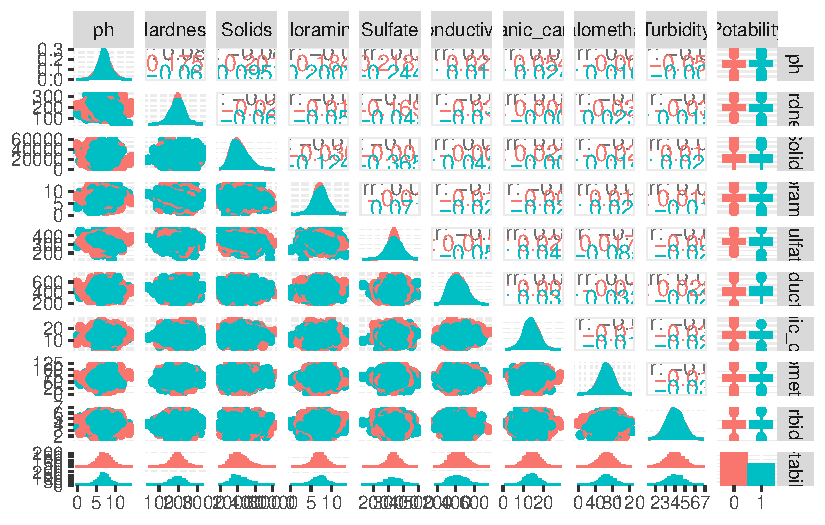
\includegraphics[keepaspectratio]{Assignment-4-Data-622-KDD_files/figure-pdf/unnamed-chunk-9-1.pdf}}

\begin{Shaded}
\begin{Highlighting}[]
\CommentTok{\#describe(fulldata)}
\FunctionTok{skim}\NormalTok{(fulldata)}
\end{Highlighting}
\end{Shaded}

\begin{longtable}[]{@{}ll@{}}
\caption{Data summary}\tabularnewline
\toprule\noalign{}
\endfirsthead
\endhead
\bottomrule\noalign{}
\endlastfoot
Name & fulldata \\
Number of rows & 3276 \\
Number of columns & 10 \\
\_\_\_\_\_\_\_\_\_\_\_\_\_\_\_\_\_\_\_\_\_\_\_ & \\
Column type frequency: & \\
factor & 1 \\
numeric & 9 \\
\_\_\_\_\_\_\_\_\_\_\_\_\_\_\_\_\_\_\_\_\_\_\_\_ & \\
Group variables & None \\
\end{longtable}

\textbf{Variable type: factor}

\begin{longtable}[]{@{}
  >{\raggedright\arraybackslash}p{(\linewidth - 10\tabcolsep) * \real{0.1944}}
  >{\raggedleft\arraybackslash}p{(\linewidth - 10\tabcolsep) * \real{0.1389}}
  >{\raggedleft\arraybackslash}p{(\linewidth - 10\tabcolsep) * \real{0.1944}}
  >{\raggedright\arraybackslash}p{(\linewidth - 10\tabcolsep) * \real{0.1111}}
  >{\raggedleft\arraybackslash}p{(\linewidth - 10\tabcolsep) * \real{0.1250}}
  >{\raggedright\arraybackslash}p{(\linewidth - 10\tabcolsep) * \real{0.2361}}@{}}
\toprule\noalign{}
\begin{minipage}[b]{\linewidth}\raggedright
skim\_variable
\end{minipage} & \begin{minipage}[b]{\linewidth}\raggedleft
n\_missing
\end{minipage} & \begin{minipage}[b]{\linewidth}\raggedleft
complete\_rate
\end{minipage} & \begin{minipage}[b]{\linewidth}\raggedright
ordered
\end{minipage} & \begin{minipage}[b]{\linewidth}\raggedleft
n\_unique
\end{minipage} & \begin{minipage}[b]{\linewidth}\raggedright
top\_counts
\end{minipage} \\
\midrule\noalign{}
\endhead
\bottomrule\noalign{}
\endlastfoot
Potability & 0 & 1 & FALSE & 2 & 0: 1998, 1: 1278 \\
\end{longtable}

\textbf{Variable type: numeric}

\begin{longtable}[]{@{}
  >{\raggedright\arraybackslash}p{(\linewidth - 20\tabcolsep) * \real{0.1509}}
  >{\raggedleft\arraybackslash}p{(\linewidth - 20\tabcolsep) * \real{0.0943}}
  >{\raggedleft\arraybackslash}p{(\linewidth - 20\tabcolsep) * \real{0.1321}}
  >{\raggedleft\arraybackslash}p{(\linewidth - 20\tabcolsep) * \real{0.0849}}
  >{\raggedleft\arraybackslash}p{(\linewidth - 20\tabcolsep) * \real{0.0755}}
  >{\raggedleft\arraybackslash}p{(\linewidth - 20\tabcolsep) * \real{0.0660}}
  >{\raggedleft\arraybackslash}p{(\linewidth - 20\tabcolsep) * \real{0.0849}}
  >{\raggedleft\arraybackslash}p{(\linewidth - 20\tabcolsep) * \real{0.0849}}
  >{\raggedleft\arraybackslash}p{(\linewidth - 20\tabcolsep) * \real{0.0849}}
  >{\raggedleft\arraybackslash}p{(\linewidth - 20\tabcolsep) * \real{0.0849}}
  >{\raggedright\arraybackslash}p{(\linewidth - 20\tabcolsep) * \real{0.0566}}@{}}
\toprule\noalign{}
\begin{minipage}[b]{\linewidth}\raggedright
skim\_variable
\end{minipage} & \begin{minipage}[b]{\linewidth}\raggedleft
n\_missing
\end{minipage} & \begin{minipage}[b]{\linewidth}\raggedleft
complete\_rate
\end{minipage} & \begin{minipage}[b]{\linewidth}\raggedleft
mean
\end{minipage} & \begin{minipage}[b]{\linewidth}\raggedleft
sd
\end{minipage} & \begin{minipage}[b]{\linewidth}\raggedleft
p0
\end{minipage} & \begin{minipage}[b]{\linewidth}\raggedleft
p25
\end{minipage} & \begin{minipage}[b]{\linewidth}\raggedleft
p50
\end{minipage} & \begin{minipage}[b]{\linewidth}\raggedleft
p75
\end{minipage} & \begin{minipage}[b]{\linewidth}\raggedleft
p100
\end{minipage} & \begin{minipage}[b]{\linewidth}\raggedright
hist
\end{minipage} \\
\midrule\noalign{}
\endhead
\bottomrule\noalign{}
\endlastfoot
ph & 491 & 0.85 & 7.08 & 1.59 & 0.00 & 6.09 & 7.04 & 8.06 & 14.00 &
▁▂▇▂▁ \\
Hardness & 0 & 1.00 & 196.37 & 32.88 & 47.43 & 176.85 & 196.97 & 216.67
& 323.12 & ▁▂▇▃▁ \\
Solids & 0 & 1.00 & 22014.09 & 8768.57 & 320.94 & 15666.69 & 20927.83 &
27332.76 & 61227.20 & ▂▇▅▁▁ \\
Chloramines & 0 & 1.00 & 7.12 & 1.58 & 0.35 & 6.13 & 7.13 & 8.11 & 13.13
& ▁▂▇▃▁ \\
Sulfate & 781 & 0.76 & 333.78 & 41.42 & 129.00 & 307.70 & 333.07 &
359.95 & 481.03 & ▁▁▇▆▁ \\
Conductivity & 0 & 1.00 & 426.21 & 80.82 & 181.48 & 365.73 & 421.88 &
481.79 & 753.34 & ▁▇▇▂▁ \\
Organic\_carbon & 0 & 1.00 & 14.28 & 3.31 & 2.20 & 12.07 & 14.22 & 16.56
& 28.30 & ▁▅▇▂▁ \\
Trihalomethanes & 162 & 0.95 & 66.40 & 16.18 & 0.74 & 55.84 & 66.62 &
77.34 & 124.00 & ▁▂▇▅▁ \\
Turbidity & 0 & 1.00 & 3.97 & 0.78 & 1.45 & 3.44 & 3.96 & 4.50 & 6.74 &
▁▅▇▃▁ \\
\end{longtable}

\begin{verbatim}
\end{verbatim}

\subsection{}\label{section-3}

\begin{verbatim}
\end{verbatim}

\subsection{}\label{section-4}

\begin{verbatim}
\end{verbatim}

\subsection{all models}\label{all-models}

\section{Train and evaluate the
Models}\label{train-and-evaluate-the-models}

\subsection{Decision Trees}\label{decision-trees}

\begin{Shaded}
\begin{Highlighting}[]
\FunctionTok{set.seed}\NormalTok{(}\DecValTok{42}\NormalTok{)}
\CommentTok{\#decision tree model}

\NormalTok{tree\_model }\OtherTok{\textless{}{-}} \FunctionTok{rpart}\NormalTok{(}
\NormalTok{  Potability }\SpecialCharTok{\textasciitilde{}}\NormalTok{ ., }
  \AttributeTok{data =}\NormalTok{ train\_data,}
  \AttributeTok{method =} \StringTok{"class"}\NormalTok{,}
  \AttributeTok{control =} \FunctionTok{rpart.control}\NormalTok{(}
    \AttributeTok{cp =} \FloatTok{0.01}\NormalTok{,}
    \AttributeTok{minsplit =} \DecValTok{30}\NormalTok{,}
    \AttributeTok{maxdepth =} \DecValTok{20}
\NormalTok{  )}
\NormalTok{)}

\NormalTok{tree\_model}
\end{Highlighting}
\end{Shaded}

\begin{verbatim}
n= 2293 

node), split, n, loss, yval, (yprob)
      * denotes terminal node

  1) root 2293 878 0 (0.3829045 0.6170955)  
    2) Sulfate< 261.2405 68  22 1 (0.6764706 0.3235294)  
      4) Solids>=18346.62 53  10 1 (0.8113208 0.1886792) *
      5) Solids< 18346.62 15   3 0 (0.2000000 0.8000000) *
    3) Sulfate>=261.2405 2225 832 0 (0.3739326 0.6260674)  
      6) Hardness< 164.3612 339 160 0 (0.4719764 0.5280236)  
       12) Chloramines>=7.911695 117  46 1 (0.6068376 0.3931624) *
       13) Chloramines< 7.911695 222  89 0 (0.4009009 0.5990991)  
         26) Solids< 16280.58 50  20 1 (0.6000000 0.4000000) *
         27) Solids>=16280.58 172  59 0 (0.3430233 0.6569767) *
      7) Hardness>=164.3612 1886 672 0 (0.3563097 0.6436903)  
       14) ph< 8.206025 1538 583 0 (0.3790637 0.6209363)  
         28) Sulfate>=365.4012 222 100 1 (0.5495495 0.4504505)  
           56) Hardness>=217.7926 70  17 1 (0.7571429 0.2428571) *
           57) Hardness< 217.7926 152  69 0 (0.4539474 0.5460526)  
            114) Chloramines< 5.44537 17   2 1 (0.8823529 0.1176471) *
            115) Chloramines>=5.44537 135  54 0 (0.4000000 0.6000000) *
         29) Sulfate< 365.4012 1316 461 0 (0.3503040 0.6496960)  
           58) Hardness>=254.399 44  16 1 (0.6363636 0.3636364) *
           59) Hardness< 254.399 1272 433 0 (0.3404088 0.6595912) *
       15) ph>=8.206025 348  89 0 (0.2557471 0.7442529) *
\end{verbatim}

\begin{Shaded}
\begin{Highlighting}[]
\FunctionTok{rpart.plot}\NormalTok{(tree\_model)}
\end{Highlighting}
\end{Shaded}

\pandocbounded{\includegraphics[keepaspectratio]{Assignment-4-Data-622-KDD_files/figure-pdf/unnamed-chunk-14-1.pdf}}

\begin{Shaded}
\begin{Highlighting}[]
\NormalTok{pred\_class }\OtherTok{\textless{}{-}} \FunctionTok{predict}\NormalTok{(tree\_model, test\_data, }\AttributeTok{type =} \StringTok{"class"}\NormalTok{)}
\NormalTok{pred\_prob }\OtherTok{\textless{}{-}} \FunctionTok{predict}\NormalTok{(tree\_model, test\_data, }\AttributeTok{type =} \StringTok{"prob"}\NormalTok{)}



\CommentTok{\#table(Predicted = pred\_class, Actual = eqtest\_data$term\_deposit\_factor)}

\CommentTok{\#mean(pred\_class == eqtest\_data$term\_deposit\_factor)}




\CommentTok{\#confusion matrix contains most metrics for classifiers}
\NormalTok{cm }\OtherTok{\textless{}{-}} \FunctionTok{confusionMatrix}\NormalTok{(pred\_class, test\_data}\SpecialCharTok{$}\NormalTok{Potability)}

\NormalTok{cm}
\end{Highlighting}
\end{Shaded}

\begin{verbatim}
Confusion Matrix and Statistics

          Reference
Prediction   1   0
         1  86  80
         0 314 503
                                        
               Accuracy : 0.5992        
                 95% CI : (0.5678, 0.63)
    No Information Rate : 0.5931        
    P-Value [Acc > NIR] : 0.3612        
                                        
                  Kappa : 0.0856        
                                        
 Mcnemar's Test P-Value : <2e-16        
                                        
            Sensitivity : 0.21500       
            Specificity : 0.86278       
         Pos Pred Value : 0.51807       
         Neg Pred Value : 0.61567       
             Prevalence : 0.40692       
         Detection Rate : 0.08749       
   Detection Prevalence : 0.16887       
      Balanced Accuracy : 0.53889       
                                        
       'Positive' Class : 1             
                                        
\end{verbatim}

\begin{Shaded}
\begin{Highlighting}[]
\CommentTok{\# calculate the F1 Score which is more useful than accuracy due to the focus on precision and recall.  (the harmonic mean of precision and recall)}
\NormalTok{precision }\OtherTok{\textless{}{-}}\NormalTok{ cm}\SpecialCharTok{$}\NormalTok{byClass[}\StringTok{"Pos Pred Value"}\NormalTok{]}
\NormalTok{recall    }\OtherTok{\textless{}{-}}\NormalTok{ cm}\SpecialCharTok{$}\NormalTok{byClass[}\StringTok{"Sensitivity"}\NormalTok{]}


\NormalTok{f1 }\OtherTok{\textless{}{-}} \DecValTok{2} \SpecialCharTok{*}\NormalTok{ (precision }\SpecialCharTok{*}\NormalTok{ recall) }\SpecialCharTok{/}\NormalTok{ (precision }\SpecialCharTok{+}\NormalTok{ recall)}
\NormalTok{f1}
\end{Highlighting}
\end{Shaded}

\begin{verbatim}
Pos Pred Value 
     0.3038869 
\end{verbatim}

\subsection{Deeper Decision Tree}\label{deeper-decision-tree}

cp = 0.001 overfit

\begin{Shaded}
\begin{Highlighting}[]
\FunctionTok{set.seed}\NormalTok{(}\DecValTok{42}\NormalTok{)}
\NormalTok{tree\_model }\OtherTok{\textless{}{-}} \FunctionTok{rpart}\NormalTok{(}
\NormalTok{  Potability }\SpecialCharTok{\textasciitilde{}}\NormalTok{ ., }
  \AttributeTok{data =}\NormalTok{ train\_data,}
  \AttributeTok{method =} \StringTok{"class"}\NormalTok{,}
  \AttributeTok{control =} \FunctionTok{rpart.control}\NormalTok{(}
    \AttributeTok{cp =} \FloatTok{0.001}\NormalTok{,}
    \AttributeTok{minsplit =} \DecValTok{30}\NormalTok{,}
    \AttributeTok{maxdepth =} \DecValTok{20}
\NormalTok{  )}
\NormalTok{)}

\NormalTok{tree\_model}
\end{Highlighting}
\end{Shaded}

\begin{verbatim}
n= 2293 

node), split, n, loss, yval, (yprob)
      * denotes terminal node

     1) root 2293 878 0 (0.38290449 0.61709551)  
       2) Sulfate< 261.2405 68  22 1 (0.67647059 0.32352941)  
         4) Solids>=18346.62 53  10 1 (0.81132075 0.18867925) *
         5) Solids< 18346.62 15   3 0 (0.20000000 0.80000000) *
       3) Sulfate>=261.2405 2225 832 0 (0.37393258 0.62606742)  
         6) Hardness< 164.3612 339 160 0 (0.47197640 0.52802360)  
          12) Chloramines>=7.911695 117  46 1 (0.60683761 0.39316239)  
            24) ph>=6.257209 77  23 1 (0.70129870 0.29870130)  
              48) Sulfate< 329.3489 35   4 1 (0.88571429 0.11428571) *
              49) Sulfate>=329.3489 42  19 1 (0.54761905 0.45238095)  
                98) Turbidity< 3.439771 11   2 1 (0.81818182 0.18181818) *
                99) Turbidity>=3.439771 31  14 0 (0.45161290 0.54838710)  
                 198) ph< 7.121211 12   4 1 (0.66666667 0.33333333) *
                 199) ph>=7.121211 19   6 0 (0.31578947 0.68421053) *
            25) ph< 6.257209 40  17 0 (0.42500000 0.57500000)  
              50) Sulfate>=330.6019 25   9 1 (0.64000000 0.36000000) *
              51) Sulfate< 330.6019 15   1 0 (0.06666667 0.93333333) *
          13) Chloramines< 7.911695 222  89 0 (0.40090090 0.59909910)  
            26) Solids< 16280.58 50  20 1 (0.60000000 0.40000000)  
              52) Solids>=13665.68 23   4 1 (0.82608696 0.17391304) *
              53) Solids< 13665.68 27  11 0 (0.40740741 0.59259259) *
            27) Solids>=16280.58 172  59 0 (0.34302326 0.65697674)  
              54) Solids>=19579.79 138  55 0 (0.39855072 0.60144928)  
               108) Sulfate< 376.8662 111  51 0 (0.45945946 0.54054054)  
                 216) Hardness>=150.5074 63  27 1 (0.57142857 0.42857143)  
                   432) ph>=5.50641 51  18 1 (0.64705882 0.35294118) *
                   433) ph< 5.50641 12   3 0 (0.25000000 0.75000000) *
                 217) Hardness< 150.5074 48  15 0 (0.31250000 0.68750000) *
               109) Sulfate>=376.8662 27   4 0 (0.14814815 0.85185185) *
              55) Solids< 19579.79 34   4 0 (0.11764706 0.88235294) *
         7) Hardness>=164.3612 1886 672 0 (0.35630965 0.64369035)  
          14) ph< 8.206025 1538 583 0 (0.37906372 0.62093628)  
            28) Sulfate>=365.4012 222 100 1 (0.54954955 0.45045045)  
              56) Hardness>=217.7926 70  17 1 (0.75714286 0.24285714)  
               112) Solids< 25287.28 50   4 1 (0.92000000 0.08000000) *
               113) Solids>=25287.28 20   7 0 (0.35000000 0.65000000) *
              57) Hardness< 217.7926 152  69 0 (0.45394737 0.54605263)  
               114) Chloramines< 5.44537 17   2 1 (0.88235294 0.11764706) *
               115) Chloramines>=5.44537 135  54 0 (0.40000000 0.60000000)  
                 230) Chloramines>=9.344868 11   2 1 (0.81818182 0.18181818) *
                 231) Chloramines< 9.344868 124  45 0 (0.36290323 0.63709677)  
                   462) Organic_carbon>=11.24699 101  42 0 (0.41584158 0.58415842)  
                     924) Organic_carbon< 13.9326 36  14 1 (0.61111111 0.38888889)  
                      1848) Chloramines< 8.04623 23   6 1 (0.73913043 0.26086957) *
                      1849) Chloramines>=8.04623 13   5 0 (0.38461538 0.61538462) *
                     925) Organic_carbon>=13.9326 65  20 0 (0.30769231 0.69230769)  
                      1850) Trihalomethanes< 71.89747 41  17 0 (0.41463415 0.58536585)  
                        3700) Hardness< 188.8751 19   8 1 (0.57894737 0.42105263) *
                        3701) Hardness>=188.8751 22   6 0 (0.27272727 0.72727273) *
                      1851) Trihalomethanes>=71.89747 24   3 0 (0.12500000 0.87500000) *
                   463) Organic_carbon< 11.24699 23   3 0 (0.13043478 0.86956522) *
            29) Sulfate< 365.4012 1316 461 0 (0.35030395 0.64969605)  
              58) Hardness>=254.399 44  16 1 (0.63636364 0.36363636)  
               116) Sulfate>=314.7838 33   8 1 (0.75757576 0.24242424) *
               117) Sulfate< 314.7838 11   3 0 (0.27272727 0.72727273) *
              59) Hardness< 254.399 1272 433 0 (0.34040881 0.65959119)  
               118) ph>=4.594908 1209 426 0 (0.35235732 0.64764268)  
                 236) ph>=7.055863 396 161 0 (0.40656566 0.59343434)  
                   472) Chloramines>=6.985978 218 107 0 (0.49082569 0.50917431)  
                     944) Conductivity< 328.9354 27   6 1 (0.77777778 0.22222222) *
                     945) Conductivity>=328.9354 191  86 0 (0.45026178 0.54973822)  
                      1890) Solids>=29267.16 32  10 1 (0.68750000 0.31250000) *
                      1891) Solids< 29267.16 159  64 0 (0.40251572 0.59748428)  
                        3782) Hardness>=187.906 122  57 0 (0.46721311 0.53278689)  
                          7564) Hardness< 198.2794 23   7 1 (0.69565217 0.30434783) *
                          7565) Hardness>=198.2794 99  41 0 (0.41414141 0.58585859)  
                           15130) Chloramines< 8.038136 52  24 1 (0.53846154 0.46153846)  
                             30260) Chloramines>=7.391049 30   8 1 (0.73333333 0.26666667)  
                               60520) Conductivity< 450.4485 17   1 1 (0.94117647 0.05882353) *
                               60521) Conductivity>=450.4485 13   6 0 (0.46153846 0.53846154) *
                             30261) Chloramines< 7.391049 22   6 0 (0.27272727 0.72727273) *
                           15131) Chloramines>=8.038136 47  13 0 (0.27659574 0.72340426)  
                             30262) Solids< 13813.33 11   4 1 (0.63636364 0.36363636) *
                             30263) Solids>=13813.33 36   6 0 (0.16666667 0.83333333) *
                        3783) Hardness< 187.906 37   7 0 (0.18918919 0.81081081) *
                   473) Chloramines< 6.985978 178  54 0 (0.30337079 0.69662921)  
                     946) Sulfate< 303.4462 27  12 1 (0.55555556 0.44444444) *
                     947) Sulfate>=303.4462 151  39 0 (0.25827815 0.74172185)  
                      1894) Solids>=16496.34 106  33 0 (0.31132075 0.68867925)  
                        3788) Chloramines>=6.365501 37  18 0 (0.48648649 0.51351351)  
                          7576) Hardness>=192.3607 25  10 1 (0.60000000 0.40000000) *
                          7577) Hardness< 192.3607 12   3 0 (0.25000000 0.75000000) *
                        3789) Chloramines< 6.365501 69  15 0 (0.21739130 0.78260870) *
                      1895) Solids< 16496.34 45   6 0 (0.13333333 0.86666667) *
                 237) ph< 7.055863 813 265 0 (0.32595326 0.67404674)  
                   474) Organic_carbon< 8.13401 28  10 1 (0.64285714 0.35714286) *
                   475) Organic_carbon>=8.13401 785 247 0 (0.31464968 0.68535032)  
                     950) ph< 7.04223 563 197 0 (0.34991119 0.65008881)  
                      1900) ph>=6.634442 160  72 0 (0.45000000 0.55000000)  
                        3800) Conductivity>=472.4072 53  22 1 (0.58490566 0.41509434)  
                          7600) Chloramines>=6.00645 42  14 1 (0.66666667 0.33333333)  
                           15200) Turbidity< 4.708821 31   7 1 (0.77419355 0.22580645) *
                           15201) Turbidity>=4.708821 11   4 0 (0.36363636 0.63636364) *
                          7601) Chloramines< 6.00645 11   3 0 (0.27272727 0.72727273) *
                        3801) Conductivity< 472.4072 107  41 0 (0.38317757 0.61682243)  
                          7602) Solids>=31070.29 18   6 1 (0.66666667 0.33333333) *
                          7603) Solids< 31070.29 89  29 0 (0.32584270 0.67415730)  
                           15206) Solids< 17469.33 31  15 1 (0.51612903 0.48387097)  
                             30412) Chloramines< 6.847432 13   3 1 (0.76923077 0.23076923) *
                             30413) Chloramines>=6.847432 18   6 0 (0.33333333 0.66666667) *
                           15207) Solids>=17469.33 58  13 0 (0.22413793 0.77586207)  
                             30414) Turbidity< 4.733707 45  13 0 (0.28888889 0.71111111)  
                               60828) Turbidity>=4.239223 10   2 1 (0.80000000 0.20000000) *
                               60829) Turbidity< 4.239223 35   5 0 (0.14285714 0.85714286) *
                             30415) Turbidity>=4.733707 13   0 0 (0.00000000 1.00000000) *
                      1901) ph< 6.634442 403 125 0 (0.31017370 0.68982630)  
                        3802) Hardness>=197.1672 204  80 0 (0.39215686 0.60784314)  
                          7604) Sulfate>=318.9145 128  63 1 (0.50781250 0.49218750)  
                           15208) Chloramines< 7.485071 80  31 1 (0.61250000 0.38750000)  
                             30416) ph< 5.53909 22   2 1 (0.90909091 0.09090909) *
                             30417) ph>=5.53909 58  29 1 (0.50000000 0.50000000)  
                               60834) Conductivity< 332.1286 14   3 1 (0.78571429 0.21428571) *
                               60835) Conductivity>=332.1286 44  18 0 (0.40909091 0.59090909)  
                                121670) Chloramines< 5.370559 10   3 1 (0.70000000 0.30000000) *
                                121671) Chloramines>=5.370559 34  11 0 (0.32352941 0.67647059)  
                                  243342) Organic_carbon< 12.78914 15   7 1 (0.53333333 0.46666667) *
                                  243343) Organic_carbon>=12.78914 19   3 0 (0.15789474 0.84210526) *
                           15209) Chloramines>=7.485071 48  16 0 (0.33333333 0.66666667)  
                             30418) Solids< 19568.21 19   7 1 (0.63157895 0.36842105) *
                             30419) Solids>=19568.21 29   4 0 (0.13793103 0.86206897) *
                          7605) Sulfate< 318.9145 76  15 0 (0.19736842 0.80263158) *
                        3803) Hardness< 197.1672 199  45 0 (0.22613065 0.77386935)  
                          7606) Solids>=35661.62 12   5 1 (0.58333333 0.41666667) *
                          7607) Solids< 35661.62 187  38 0 (0.20320856 0.79679144)  
                           15214) ph>=5.751502 115  31 0 (0.26956522 0.73043478)  
                             30428) Hardness>=185.4236 49  20 0 (0.40816327 0.59183673)  
                               60856) Hardness< 189.2005 20   8 1 (0.60000000 0.40000000) *
                               60857) Hardness>=189.2005 29   8 0 (0.27586207 0.72413793) *
                             30429) Hardness< 185.4236 66  11 0 (0.16666667 0.83333333) *
                           15215) ph< 5.751502 72   7 0 (0.09722222 0.90277778) *
                     951) ph>=7.04223 222  50 0 (0.22522523 0.77477477)  
                      1902) Sulfate< 319.1 58  20 0 (0.34482759 0.65517241)  
                        3804) Chloramines< 6.590676 17   7 1 (0.58823529 0.41176471) *
                        3805) Chloramines>=6.590676 41  10 0 (0.24390244 0.75609756)  
                          7610) Sulfate>=310.1858 11   5 1 (0.54545455 0.45454545) *
                          7611) Sulfate< 310.1858 30   4 0 (0.13333333 0.86666667) *
                      1903) Sulfate>=319.1 164  30 0 (0.18292683 0.81707317) *
               119) ph< 4.594908 63   7 0 (0.11111111 0.88888889) *
          15) ph>=8.206025 348  89 0 (0.25574713 0.74425287)  
            30) Sulfate< 284.1368 14   3 1 (0.78571429 0.21428571) *
            31) Sulfate>=284.1368 334  78 0 (0.23353293 0.76646707)  
              62) Chloramines>=8.423856 44  20 0 (0.45454545 0.54545455)  
               124) Sulfate< 349.7264 27  10 1 (0.62962963 0.37037037) *
               125) Sulfate>=349.7264 17   3 0 (0.17647059 0.82352941) *
              63) Chloramines< 8.423856 290  58 0 (0.20000000 0.80000000)  
               126) Organic_carbon< 12.58131 70  24 0 (0.34285714 0.65714286)  
                 252) Organic_carbon>=12.02412 16   5 1 (0.68750000 0.31250000) *
                 253) Organic_carbon< 12.02412 54  13 0 (0.24074074 0.75925926) *
               127) Organic_carbon>=12.58131 220  34 0 (0.15454545 0.84545455)  
                 254) Solids>=13653.4 169  34 0 (0.20118343 0.79881657)  
                   508) Hardness< 194.1059 41  14 0 (0.34146341 0.65853659)  
                    1016) Organic_carbon< 14.52538 13   4 1 (0.69230769 0.30769231) *
                    1017) Organic_carbon>=14.52538 28   5 0 (0.17857143 0.82142857) *
                   509) Hardness>=194.1059 128  20 0 (0.15625000 0.84375000) *
                 255) Solids< 13653.4 51   0 0 (0.00000000 1.00000000) *
\end{verbatim}

\begin{Shaded}
\begin{Highlighting}[]
\FunctionTok{rpart.plot}\NormalTok{(tree\_model)}
\end{Highlighting}
\end{Shaded}

\begin{verbatim}
Warning: labs do not fit even at cex 0.15, there may be some overplotting
\end{verbatim}

\pandocbounded{\includegraphics[keepaspectratio]{Assignment-4-Data-622-KDD_files/figure-pdf/unnamed-chunk-15-1.pdf}}

\begin{Shaded}
\begin{Highlighting}[]
\NormalTok{pred\_class }\OtherTok{\textless{}{-}} \FunctionTok{predict}\NormalTok{(tree\_model, test\_data, }\AttributeTok{type =} \StringTok{"class"}\NormalTok{)}




\FunctionTok{table}\NormalTok{(}\AttributeTok{Predicted =}\NormalTok{ pred\_class, }\AttributeTok{Actual =}\NormalTok{ test\_data}\SpecialCharTok{$}\NormalTok{Potability)}
\end{Highlighting}
\end{Shaded}

\begin{verbatim}
         Actual
Predicted   1   0
        1 185 193
        0 215 390
\end{verbatim}

\begin{Shaded}
\begin{Highlighting}[]
\FunctionTok{mean}\NormalTok{(pred\_class }\SpecialCharTok{==}\NormalTok{ test\_data}\SpecialCharTok{$}\NormalTok{Potability)}
\end{Highlighting}
\end{Shaded}

\begin{verbatim}
[1] 0.584944
\end{verbatim}

\begin{Shaded}
\begin{Highlighting}[]
\CommentTok{\#confusionMatrix(pred\_class$class, actual, positive = "1")}
\NormalTok{cm }\OtherTok{\textless{}{-}} \FunctionTok{confusionMatrix}\NormalTok{(pred\_class, test\_data}\SpecialCharTok{$}\NormalTok{Potability)}
\NormalTok{cm}
\end{Highlighting}
\end{Shaded}

\begin{verbatim}
Confusion Matrix and Statistics

          Reference
Prediction   1   0
         1 185 193
         0 215 390
                                         
               Accuracy : 0.5849         
                 95% CI : (0.5534, 0.616)
    No Information Rate : 0.5931         
    P-Value [Acc > NIR] : 0.7099         
                                         
                  Kappa : 0.1326         
                                         
 Mcnemar's Test P-Value : 0.2985         
                                         
            Sensitivity : 0.4625         
            Specificity : 0.6690         
         Pos Pred Value : 0.4894         
         Neg Pred Value : 0.6446         
             Prevalence : 0.4069         
         Detection Rate : 0.1882         
   Detection Prevalence : 0.3845         
      Balanced Accuracy : 0.5657         
                                         
       'Positive' Class : 1              
                                         
\end{verbatim}

\begin{Shaded}
\begin{Highlighting}[]
\NormalTok{precision }\OtherTok{\textless{}{-}}\NormalTok{ cm}\SpecialCharTok{$}\NormalTok{byClass[}\StringTok{"Pos Pred Value"}\NormalTok{]}
\NormalTok{recall    }\OtherTok{\textless{}{-}}\NormalTok{ cm}\SpecialCharTok{$}\NormalTok{byClass[}\StringTok{"Sensitivity"}\NormalTok{]}


\NormalTok{f1\_tree }\OtherTok{\textless{}{-}} \DecValTok{2} \SpecialCharTok{*}\NormalTok{ (precision }\SpecialCharTok{*}\NormalTok{ recall) }\SpecialCharTok{/}\NormalTok{ (precision }\SpecialCharTok{+}\NormalTok{ recall)}
\NormalTok{f1\_tree}
\end{Highlighting}
\end{Shaded}

\begin{verbatim}
Pos Pred Value 
     0.4755784 
\end{verbatim}

\begin{verbatim}
\end{verbatim}

\begin{verbatim}
\end{verbatim}

\subsection{Random forest}\label{random-forest}

\begin{Shaded}
\begin{Highlighting}[]
\FunctionTok{set.seed}\NormalTok{(}\DecValTok{42}\NormalTok{)}
\CommentTok{\#random forest model}

\NormalTok{rf\_model }\OtherTok{\textless{}{-}} \FunctionTok{randomForest}\NormalTok{(}
\NormalTok{  Potability }\SpecialCharTok{\textasciitilde{}}\NormalTok{ ., }
  \AttributeTok{data =}\NormalTok{ train\_data,}
  
  \AttributeTok{ntree =} \DecValTok{500}\NormalTok{,}
  \AttributeTok{importance =} \ConstantTok{TRUE}
\NormalTok{)}

\NormalTok{forrest\_pred\_class }\OtherTok{\textless{}{-}} \FunctionTok{predict}\NormalTok{(rf\_model, test\_data, }\AttributeTok{type =} \StringTok{"class"}\NormalTok{)}
\NormalTok{forrest\_pred\_prob }\OtherTok{\textless{}{-}} \FunctionTok{predict}\NormalTok{(rf\_model, test\_data, }\AttributeTok{type =} \StringTok{"prob"}\NormalTok{)}

\NormalTok{rf\_model}
\end{Highlighting}
\end{Shaded}

\begin{verbatim}

Call:
 randomForest(formula = Potability ~ ., data = train_data, ntree = 500,      importance = TRUE) 
               Type of random forest: classification
                     Number of trees: 500
No. of variables tried at each split: 3

        OOB estimate of  error rate: 32.53%
Confusion matrix:
    1    0 class.error
1 291  587   0.6685649
0 159 1256   0.1123675
\end{verbatim}

\begin{Shaded}
\begin{Highlighting}[]
\FunctionTok{table}\NormalTok{(}\AttributeTok{Predicted =}\NormalTok{ forrest\_pred\_class, }\AttributeTok{Actual =}\NormalTok{ test\_data}\SpecialCharTok{$}\NormalTok{Potability)}
\end{Highlighting}
\end{Shaded}

\begin{verbatim}
         Actual
Predicted   1   0
        1 151  70
        0 249 513
\end{verbatim}

\begin{Shaded}
\begin{Highlighting}[]
\FunctionTok{mean}\NormalTok{(forrest\_pred\_class }\SpecialCharTok{==}\NormalTok{ test\_data}\SpecialCharTok{$}\NormalTok{Potability)}
\end{Highlighting}
\end{Shaded}

\begin{verbatim}
[1] 0.6754832
\end{verbatim}

\begin{Shaded}
\begin{Highlighting}[]
\NormalTok{cm }\OtherTok{\textless{}{-}} \FunctionTok{confusionMatrix}\NormalTok{(forrest\_pred\_class, test\_data}\SpecialCharTok{$}\NormalTok{Potability)}

\NormalTok{cm}
\end{Highlighting}
\end{Shaded}

\begin{verbatim}
Confusion Matrix and Statistics

          Reference
Prediction   1   0
         1 151  70
         0 249 513
                                          
               Accuracy : 0.6755          
                 95% CI : (0.6452, 0.7047)
    No Information Rate : 0.5931          
    P-Value [Acc > NIR] : 5.997e-08       
                                          
                  Kappa : 0.2769          
                                          
 Mcnemar's Test P-Value : < 2.2e-16       
                                          
            Sensitivity : 0.3775          
            Specificity : 0.8799          
         Pos Pred Value : 0.6833          
         Neg Pred Value : 0.6732          
             Prevalence : 0.4069          
         Detection Rate : 0.1536          
   Detection Prevalence : 0.2248          
      Balanced Accuracy : 0.6287          
                                          
       'Positive' Class : 1               
                                          
\end{verbatim}

\begin{Shaded}
\begin{Highlighting}[]
\NormalTok{precision }\OtherTok{\textless{}{-}}\NormalTok{ cm}\SpecialCharTok{$}\NormalTok{byClass[}\StringTok{"Pos Pred Value"}\NormalTok{]}
\NormalTok{recall    }\OtherTok{\textless{}{-}}\NormalTok{ cm}\SpecialCharTok{$}\NormalTok{byClass[}\StringTok{"Sensitivity"}\NormalTok{]}


\NormalTok{f1\_rf }\OtherTok{\textless{}{-}} \DecValTok{2} \SpecialCharTok{*}\NormalTok{ (precision }\SpecialCharTok{*}\NormalTok{ recall) }\SpecialCharTok{/}\NormalTok{ (precision }\SpecialCharTok{+}\NormalTok{ recall)}
\NormalTok{f1\_rf}
\end{Highlighting}
\end{Shaded}

\begin{verbatim}
Pos Pred Value 
     0.4863124 
\end{verbatim}

\begin{Shaded}
\begin{Highlighting}[]
\FunctionTok{varImpPlot}\NormalTok{(rf\_model)}
\end{Highlighting}
\end{Shaded}

\pandocbounded{\includegraphics[keepaspectratio]{Assignment-4-Data-622-KDD_files/figure-pdf/unnamed-chunk-16-1.pdf}}

surprisingly model performance is roughly equal to just one decision
tree

kappa 0.4894, sensitivity 0.8791, specificity 0.6105 accuracy 0.7446

F1 0.7116969

\begin{verbatim}
\end{verbatim}

\begin{verbatim}
\end{verbatim}

\begin{verbatim}
Accuracy : 0.7453, Kappa : 0.4909, Sensitivity : 0.8827, Specificity : 0.6083
specificity decreased
\end{verbatim}

\subsection{Tuned Random Forest}\label{tuned-random-forest}

\begin{verbatim}

  
\end{verbatim}

\subsection{Adaboost}\label{adaboost}

\begin{Shaded}
\begin{Highlighting}[]
\CommentTok{\#adaptive boosting model}


\CommentTok{\#ada\_partdata \textless{}{-}partdata |\textgreater{}  dplyr::select({-}y, {-}term\_deposit, {-}default)}
\CommentTok{\#ada\_partdata[] \textless{}{-} lapply(ada\_partdata, function(x) \{}
\CommentTok{\#  if (is.character(x)) factor(x) else x}
\CommentTok{\#\})}

\DocumentationTok{\#\#ada\_partdata$default \textless{}{-} factor(ada\_partdata$default, levels = c("no", "yes", "unknown"))}
  
\FunctionTok{set.seed}\NormalTok{(}\DecValTok{42}\NormalTok{)}



\NormalTok{ada\_model }\OtherTok{\textless{}{-}} \FunctionTok{boosting}\NormalTok{(}
\NormalTok{  Potability }\SpecialCharTok{\textasciitilde{}}\NormalTok{ .,}
  \AttributeTok{data =}\NormalTok{ train\_data,}
  \AttributeTok{mfinal =} \DecValTok{100}\NormalTok{,     }\CommentTok{\# number of boosting iterations}
  \AttributeTok{boos =} \ConstantTok{TRUE}
\NormalTok{)}

\CommentTok{\#ada\_model}

\NormalTok{ada\_pred }\OtherTok{\textless{}{-}} \FunctionTok{predict}\NormalTok{(ada\_model, test\_data)}

\NormalTok{ada\_pred}\SpecialCharTok{$}\NormalTok{class }\OtherTok{\textless{}{-}} \FunctionTok{factor}\NormalTok{(}
\NormalTok{  ada\_pred}\SpecialCharTok{$}\NormalTok{class,}
  \AttributeTok{levels =} \FunctionTok{levels}\NormalTok{(test\_data}\SpecialCharTok{$}\NormalTok{Potability)}
\NormalTok{)}

\NormalTok{cm }\OtherTok{\textless{}{-}} \FunctionTok{confusionMatrix}\NormalTok{(ada\_pred}\SpecialCharTok{$}\NormalTok{class, test\_data}\SpecialCharTok{$}\NormalTok{Potability)}

\NormalTok{cm}
\end{Highlighting}
\end{Shaded}

\begin{verbatim}
Confusion Matrix and Statistics

          Reference
Prediction   1   0
         1 169 111
         0 231 472
                                          
               Accuracy : 0.6521          
                 95% CI : (0.6214, 0.6819)
    No Information Rate : 0.5931          
    P-Value [Acc > NIR] : 8.357e-05       
                                          
                  Kappa : 0.2436          
                                          
 Mcnemar's Test P-Value : 1.236e-10       
                                          
            Sensitivity : 0.4225          
            Specificity : 0.8096          
         Pos Pred Value : 0.6036          
         Neg Pred Value : 0.6714          
             Prevalence : 0.4069          
         Detection Rate : 0.1719          
   Detection Prevalence : 0.2848          
      Balanced Accuracy : 0.6161          
                                          
       'Positive' Class : 1               
                                          
\end{verbatim}

\begin{Shaded}
\begin{Highlighting}[]
\NormalTok{precision }\OtherTok{\textless{}{-}}\NormalTok{ cm}\SpecialCharTok{$}\NormalTok{byClass[}\StringTok{"Pos Pred Value"}\NormalTok{]}
\NormalTok{recall    }\OtherTok{\textless{}{-}}\NormalTok{ cm}\SpecialCharTok{$}\NormalTok{byClass[}\StringTok{"Sensitivity"}\NormalTok{]}


\NormalTok{f1\_ada }\OtherTok{\textless{}{-}} \DecValTok{2} \SpecialCharTok{*}\NormalTok{ (precision }\SpecialCharTok{*}\NormalTok{ recall) }\SpecialCharTok{/}\NormalTok{ (precision }\SpecialCharTok{+}\NormalTok{ recall)}
\NormalTok{f1\_ada}
\end{Highlighting}
\end{Shaded}

\begin{verbatim}
Pos Pred Value 
     0.4970588 
\end{verbatim}

\begin{Shaded}
\begin{Highlighting}[]
\FunctionTok{sort}\NormalTok{(ada\_model}\SpecialCharTok{$}\NormalTok{importance, }\AttributeTok{decreasing =} \ConstantTok{TRUE}\NormalTok{)}
\end{Highlighting}
\end{Shaded}

\begin{verbatim}
             ph         Sulfate        Hardness          Solids     Chloramines 
      16.769479       14.418847       13.255398       11.705347       11.301376 
   Conductivity Trihalomethanes  Organic_carbon       Turbidity 
       8.890219        8.409151        7.949138        7.301046 
\end{verbatim}

\subsection{SVM: Radial Basis kernel}\label{svm-radial-basis-kernel}

\begin{Shaded}
\begin{Highlighting}[]
\FunctionTok{set.seed}\NormalTok{(}\DecValTok{42}\NormalTok{)}
\CommentTok{\#SVM model radial basis kernel}




\NormalTok{SVM\_rbf\_model }\OtherTok{\textless{}{-}} \FunctionTok{ksvm}\NormalTok{(}
\NormalTok{  Potability }\SpecialCharTok{\textasciitilde{}}\NormalTok{ ., }
  \AttributeTok{data =}\NormalTok{ train\_data,}
  \AttributeTok{kernel =} \StringTok{"rbfdot"}
\NormalTok{)}

\NormalTok{SVM\_rbf\_model}
\end{Highlighting}
\end{Shaded}

\begin{verbatim}
Support Vector Machine object of class "ksvm" 

SV type: C-svc  (classification) 
 parameter : cost C = 1 

Gaussian Radial Basis kernel function. 
 Hyperparameter : sigma =  0.0836255427875869 

Number of Support Vectors : 1711 

Objective Function Value : -1500.678 
Training error : 0.280855 
\end{verbatim}

\begin{Shaded}
\begin{Highlighting}[]
\NormalTok{rbf\_pred\_class }\OtherTok{\textless{}{-}} \FunctionTok{predict}\NormalTok{(SVM\_rbf\_model, test\_data, }\AttributeTok{type =} \StringTok{"response"}\NormalTok{)}




\CommentTok{\#table(Predicted = rbf\_pred\_class, Actual = eqtest\_data$term\_deposit\_factor)}



\NormalTok{cm }\OtherTok{\textless{}{-}} \FunctionTok{confusionMatrix}\NormalTok{(rbf\_pred\_class, test\_data}\SpecialCharTok{$}\NormalTok{Potability)}

\NormalTok{cm}
\end{Highlighting}
\end{Shaded}

\begin{verbatim}
Confusion Matrix and Statistics

          Reference
Prediction   1   0
         1 121  34
         0 279 549
                                          
               Accuracy : 0.6816          
                 95% CI : (0.6514, 0.7106)
    No Information Rate : 0.5931          
    P-Value [Acc > NIR] : 6.16e-09        
                                          
                  Kappa : 0.2702          
                                          
 Mcnemar's Test P-Value : < 2.2e-16       
                                          
            Sensitivity : 0.3025          
            Specificity : 0.9417          
         Pos Pred Value : 0.7806          
         Neg Pred Value : 0.6630          
             Prevalence : 0.4069          
         Detection Rate : 0.1231          
   Detection Prevalence : 0.1577          
      Balanced Accuracy : 0.6221          
                                          
       'Positive' Class : 1               
                                          
\end{verbatim}

\begin{Shaded}
\begin{Highlighting}[]
\CommentTok{\#calculate f1 from precision and recall}
\NormalTok{precision }\OtherTok{\textless{}{-}}\NormalTok{ cm}\SpecialCharTok{$}\NormalTok{byClass[}\StringTok{"Pos Pred Value"}\NormalTok{]}
\NormalTok{recall    }\OtherTok{\textless{}{-}}\NormalTok{ cm}\SpecialCharTok{$}\NormalTok{byClass[}\StringTok{"Sensitivity"}\NormalTok{]}


\NormalTok{f1 }\OtherTok{\textless{}{-}} \DecValTok{2} \SpecialCharTok{*}\NormalTok{ (precision }\SpecialCharTok{*}\NormalTok{ recall) }\SpecialCharTok{/}\NormalTok{ (precision }\SpecialCharTok{+}\NormalTok{ recall)}
\NormalTok{f1}
\end{Highlighting}
\end{Shaded}

\begin{verbatim}
Pos Pred Value 
      0.436036 
\end{verbatim}

radial f1

\subsection{SVM: Linear kernel}\label{svm-linear-kernel}

\begin{Shaded}
\begin{Highlighting}[]
\FunctionTok{set.seed}\NormalTok{(}\DecValTok{42}\NormalTok{)}
\CommentTok{\#SVM model}



\NormalTok{SVM\_lin\_model }\OtherTok{\textless{}{-}} \FunctionTok{ksvm}\NormalTok{(}
\NormalTok{  Potability }\SpecialCharTok{\textasciitilde{}}\NormalTok{ ., }
  \AttributeTok{data =}\NormalTok{ train\_data,}
  \AttributeTok{kernel =} \StringTok{"vanilladot"}
\NormalTok{)}
\end{Highlighting}
\end{Shaded}

\begin{verbatim}
 Setting default kernel parameters  
\end{verbatim}

\begin{Shaded}
\begin{Highlighting}[]
\NormalTok{SVM\_lin\_model}
\end{Highlighting}
\end{Shaded}

\begin{verbatim}
Support Vector Machine object of class "ksvm" 

SV type: C-svc  (classification) 
 parameter : cost C = 1 

Linear (vanilla) kernel function. 

Number of Support Vectors : 1899 

Objective Function Value : -1756 
Training error : 0.382904 
\end{verbatim}

\begin{Shaded}
\begin{Highlighting}[]
\NormalTok{lin\_pred\_class }\OtherTok{\textless{}{-}} \FunctionTok{predict}\NormalTok{(SVM\_lin\_model, test\_data, }\AttributeTok{type =} \StringTok{"response"}\NormalTok{)}




\CommentTok{\#table(Predicted = rbf\_pred\_class, Actual = eqtest\_data$term\_deposit\_factor)}



\NormalTok{cm }\OtherTok{\textless{}{-}} \FunctionTok{confusionMatrix}\NormalTok{(lin\_pred\_class, test\_data}\SpecialCharTok{$}\NormalTok{Potability)}

\NormalTok{cm}
\end{Highlighting}
\end{Shaded}

\begin{verbatim}
Confusion Matrix and Statistics

          Reference
Prediction   1   0
         1   0   0
         0 400 583
                                         
               Accuracy : 0.5931         
                 95% CI : (0.5616, 0.624)
    No Information Rate : 0.5931         
    P-Value [Acc > NIR] : 0.5137         
                                         
                  Kappa : 0              
                                         
 Mcnemar's Test P-Value : <2e-16         
                                         
            Sensitivity : 0.0000         
            Specificity : 1.0000         
         Pos Pred Value :    NaN         
         Neg Pred Value : 0.5931         
             Prevalence : 0.4069         
         Detection Rate : 0.0000         
   Detection Prevalence : 0.0000         
      Balanced Accuracy : 0.5000         
                                         
       'Positive' Class : 1              
                                         
\end{verbatim}

\begin{Shaded}
\begin{Highlighting}[]
\CommentTok{\#calculate f1 from precision and recall}
\NormalTok{precision }\OtherTok{\textless{}{-}}\NormalTok{ cm}\SpecialCharTok{$}\NormalTok{byClass[}\StringTok{"Pos Pred Value"}\NormalTok{]}
\NormalTok{recall    }\OtherTok{\textless{}{-}}\NormalTok{ cm}\SpecialCharTok{$}\NormalTok{byClass[}\StringTok{"Sensitivity"}\NormalTok{]}


\NormalTok{f1 }\OtherTok{\textless{}{-}} \DecValTok{2} \SpecialCharTok{*}\NormalTok{ (precision }\SpecialCharTok{*}\NormalTok{ recall) }\SpecialCharTok{/}\NormalTok{ (precision }\SpecialCharTok{+}\NormalTok{ recall)}
\NormalTok{f1}
\end{Highlighting}
\end{Shaded}

\begin{verbatim}
Pos Pred Value 
           NaN 
\end{verbatim}

linear f1 0.697559

\begin{verbatim}
\end{verbatim}

\subsection{SVM: hyperbolic tangent sigmoid
kernel}\label{svm-hyperbolic-tangent-sigmoid-kernel}

\begin{Shaded}
\begin{Highlighting}[]
\FunctionTok{set.seed}\NormalTok{(}\DecValTok{42}\NormalTok{)}
\CommentTok{\#SVM model}



\NormalTok{SVM\_tanh\_model }\OtherTok{\textless{}{-}} \FunctionTok{ksvm}\NormalTok{(}
\NormalTok{  Potability }\SpecialCharTok{\textasciitilde{}}\NormalTok{ ., }
  \AttributeTok{data =}\NormalTok{ train\_data,}
  \AttributeTok{kernel =} \StringTok{"tanhdot"}
\NormalTok{)}
\end{Highlighting}
\end{Shaded}

\begin{verbatim}
 Setting default kernel parameters  
\end{verbatim}

\begin{Shaded}
\begin{Highlighting}[]
\NormalTok{SVM\_tanh\_model}
\end{Highlighting}
\end{Shaded}

\begin{verbatim}
Support Vector Machine object of class "ksvm" 

SV type: C-svc  (classification) 
 parameter : cost C = 1 

Hyperbolic Tangent kernel function. 
 Hyperparameters : scale =  1  offset =  1 

Number of Support Vectors : 1315 

Objective Function Value : -27507.11 
Training error : 0.57174 
\end{verbatim}

\begin{Shaded}
\begin{Highlighting}[]
\NormalTok{tanh\_pred\_class }\OtherTok{\textless{}{-}} \FunctionTok{predict}\NormalTok{(SVM\_tanh\_model, test\_data, }\AttributeTok{type =} \StringTok{"response"}\NormalTok{)}




\CommentTok{\#table(Predicted = rbf\_pred\_class, Actual = eqtest\_data$term\_deposit\_factor)}



\NormalTok{cm }\OtherTok{\textless{}{-}} \FunctionTok{confusionMatrix}\NormalTok{(tanh\_pred\_class, test\_data}\SpecialCharTok{$}\NormalTok{Potability)}

\NormalTok{cm}
\end{Highlighting}
\end{Shaded}

\begin{verbatim}
Confusion Matrix and Statistics

          Reference
Prediction   1   0
         1 105 262
         0 295 321
                                         
               Accuracy : 0.4334         
                 95% CI : (0.4021, 0.465)
    No Information Rate : 0.5931         
    P-Value [Acc > NIR] : 1.0000         
                                         
                  Kappa : -0.1894        
                                         
 Mcnemar's Test P-Value : 0.1751         
                                         
            Sensitivity : 0.2625         
            Specificity : 0.5506         
         Pos Pred Value : 0.2861         
         Neg Pred Value : 0.5211         
             Prevalence : 0.4069         
         Detection Rate : 0.1068         
   Detection Prevalence : 0.3733         
      Balanced Accuracy : 0.4066         
                                         
       'Positive' Class : 1              
                                         
\end{verbatim}

\begin{Shaded}
\begin{Highlighting}[]
\CommentTok{\#calculate f1 from precision and recall}
\NormalTok{precision }\OtherTok{\textless{}{-}}\NormalTok{ cm}\SpecialCharTok{$}\NormalTok{byClass[}\StringTok{"Pos Pred Value"}\NormalTok{]}
\NormalTok{recall    }\OtherTok{\textless{}{-}}\NormalTok{ cm}\SpecialCharTok{$}\NormalTok{byClass[}\StringTok{"Sensitivity"}\NormalTok{]}


\NormalTok{f1 }\OtherTok{\textless{}{-}} \DecValTok{2} \SpecialCharTok{*}\NormalTok{ (precision }\SpecialCharTok{*}\NormalTok{ recall) }\SpecialCharTok{/}\NormalTok{ (precision }\SpecialCharTok{+}\NormalTok{ recall)}
\NormalTok{f1}
\end{Highlighting}
\end{Shaded}

\begin{verbatim}
Pos Pred Value 
      0.273794 
\end{verbatim}

tanh f1 0.5557

radial is the best

\subsection{Cost Parameters SVM}\label{cost-parameters-svm}

Cost Parameter based on accuracy

\begin{Shaded}
\begin{Highlighting}[]
\NormalTok{cost\_values }\OtherTok{\textless{}{-}} \FunctionTok{c}\NormalTok{(}\FunctionTok{seq}\NormalTok{(}\AttributeTok{from=}\DecValTok{1}\NormalTok{, }\AttributeTok{to  =} \DecValTok{26}\NormalTok{, }\AttributeTok{by =} \DecValTok{5}\NormalTok{))}
\NormalTok{f1\_values }\OtherTok{\textless{}{-}} \FunctionTok{sapply}\NormalTok{(cost\_values, }\ControlFlowTok{function}\NormalTok{(x)\{}
\NormalTok{  SVM\_rbf\_model }\OtherTok{\textless{}{-}} \FunctionTok{ksvm}\NormalTok{(}
\NormalTok{  Potability }\SpecialCharTok{\textasciitilde{}}\NormalTok{ ., }
  \AttributeTok{data =}\NormalTok{ train\_data,}
  \AttributeTok{kernel =} \StringTok{"rbfdot"}\NormalTok{, }\AttributeTok{C =}\NormalTok{ x}
\NormalTok{)}
\NormalTok{  rbf\_pred }\OtherTok{\textless{}{-}} \FunctionTok{predict}\NormalTok{(SVM\_rbf\_model, test\_data, }\AttributeTok{type =} \StringTok{"response"}\NormalTok{)}
  \CommentTok{\#agree \textless{}{-} ifelse(rbf\_pred == eqtest\_data$term\_deposit\_factor, 1, 0)}
  \CommentTok{\#accuracy \textless{}{-}  sum(agree) / nrow(eqtest\_data)}
  
\NormalTok{   cm }\OtherTok{\textless{}{-}} \FunctionTok{confusionMatrix}\NormalTok{(rbf\_pred, test\_data}\SpecialCharTok{$}\NormalTok{Potability)}

\CommentTok{\#cm}

\CommentTok{\#calculate f1 from precision and recall}
\NormalTok{precision }\OtherTok{\textless{}{-}}\NormalTok{ cm}\SpecialCharTok{$}\NormalTok{byClass[}\StringTok{"Pos Pred Value"}\NormalTok{]}
\NormalTok{recall    }\OtherTok{\textless{}{-}}\NormalTok{ cm}\SpecialCharTok{$}\NormalTok{byClass[}\StringTok{"Sensitivity"}\NormalTok{]}


\NormalTok{f1 }\OtherTok{\textless{}{-}} \DecValTok{2} \SpecialCharTok{*}\NormalTok{ (precision }\SpecialCharTok{*}\NormalTok{ recall) }\SpecialCharTok{/}\NormalTok{ (precision }\SpecialCharTok{+}\NormalTok{ recall)}
  
  \FunctionTok{return}\NormalTok{ (f1)}
\NormalTok{\})}

\FunctionTok{plot}\NormalTok{(cost\_values, f1\_values, }\AttributeTok{type =} \StringTok{"b"}\NormalTok{)}
\end{Highlighting}
\end{Shaded}

\pandocbounded{\includegraphics[keepaspectratio]{Assignment-4-Data-622-KDD_files/figure-pdf/unnamed-chunk-23-1.pdf}}

cost parameter of 16 had the highest F1 score. This was used as the best
SVM model to compare to the other models.

\begin{Shaded}
\begin{Highlighting}[]
\FunctionTok{set.seed}\NormalTok{(}\DecValTok{42}\NormalTok{)}
\CommentTok{\#SVM model}



\NormalTok{SVM\_rbf\_model }\OtherTok{\textless{}{-}} \FunctionTok{ksvm}\NormalTok{(}
\NormalTok{  Potability }\SpecialCharTok{\textasciitilde{}}\NormalTok{ ., }
  \AttributeTok{data =}\NormalTok{ train\_data,}
  \AttributeTok{kernel =} \StringTok{"rbfdot"}\NormalTok{, }\AttributeTok{C =} \DecValTok{16}
\NormalTok{)}

\NormalTok{SVM\_rbf\_model}
\end{Highlighting}
\end{Shaded}

\begin{verbatim}
Support Vector Machine object of class "ksvm" 

SV type: C-svc  (classification) 
 parameter : cost C = 16 

Gaussian Radial Basis kernel function. 
 Hyperparameter : sigma =  0.0836255427875869 

Number of Support Vectors : 1568 

Objective Function Value : -17313.53 
Training error : 0.175752 
\end{verbatim}

\begin{Shaded}
\begin{Highlighting}[]
\NormalTok{rbf\_pred\_class }\OtherTok{\textless{}{-}} \FunctionTok{predict}\NormalTok{(SVM\_rbf\_model, test\_data, }\AttributeTok{type =} \StringTok{"response"}\NormalTok{)}




\CommentTok{\#table(Predicted = rbf\_pred\_class, Actual = eqtest\_data$term\_deposit\_factor)}



\NormalTok{cm }\OtherTok{\textless{}{-}} \FunctionTok{confusionMatrix}\NormalTok{(rbf\_pred\_class, test\_data}\SpecialCharTok{$}\NormalTok{Potability)}

\NormalTok{cm}
\end{Highlighting}
\end{Shaded}

\begin{verbatim}
Confusion Matrix and Statistics

          Reference
Prediction   1   0
         1 177 117
         0 223 466
                                          
               Accuracy : 0.6541          
                 95% CI : (0.6234, 0.6839)
    No Information Rate : 0.5931          
    P-Value [Acc > NIR] : 4.880e-05       
                                          
                  Kappa : 0.2523          
                                          
 Mcnemar's Test P-Value : 1.238e-08       
                                          
            Sensitivity : 0.4425          
            Specificity : 0.7993          
         Pos Pred Value : 0.6020          
         Neg Pred Value : 0.6763          
             Prevalence : 0.4069          
         Detection Rate : 0.1801          
   Detection Prevalence : 0.2991          
      Balanced Accuracy : 0.6209          
                                          
       'Positive' Class : 1               
                                          
\end{verbatim}

\begin{Shaded}
\begin{Highlighting}[]
\CommentTok{\#calculate f1 from precision and recall}
\NormalTok{precision }\OtherTok{\textless{}{-}}\NormalTok{ cm}\SpecialCharTok{$}\NormalTok{byClass[}\StringTok{"Pos Pred Value"}\NormalTok{]}
\NormalTok{recall    }\OtherTok{\textless{}{-}}\NormalTok{ cm}\SpecialCharTok{$}\NormalTok{byClass[}\StringTok{"Sensitivity"}\NormalTok{]}


\NormalTok{f1\_svm }\OtherTok{\textless{}{-}} \DecValTok{2} \SpecialCharTok{*}\NormalTok{ (precision }\SpecialCharTok{*}\NormalTok{ recall) }\SpecialCharTok{/}\NormalTok{ (precision }\SpecialCharTok{+}\NormalTok{ recall)}
\NormalTok{f1\_svm}
\end{Highlighting}
\end{Shaded}

\begin{verbatim}
Pos Pred Value 
     0.5100865 
\end{verbatim}

\begin{Shaded}
\begin{Highlighting}[]
\NormalTok{train\_data}\SpecialCharTok{$}\NormalTok{Potability }\OtherTok{\textless{}{-}} \FunctionTok{factor}\NormalTok{(train\_data}\SpecialCharTok{$}\NormalTok{Potability, }\AttributeTok{levels =} \FunctionTok{c}\NormalTok{(}\DecValTok{0}\NormalTok{, }\DecValTok{1}\NormalTok{))}
\NormalTok{test\_data}\SpecialCharTok{$}\NormalTok{Potability }\OtherTok{\textless{}{-}} \FunctionTok{factor}\NormalTok{(test\_data}\SpecialCharTok{$}\NormalTok{Potability, }\AttributeTok{levels =} \FunctionTok{c}\NormalTok{(}\DecValTok{0}\NormalTok{, }\DecValTok{1}\NormalTok{))}
\NormalTok{train\_data}\SpecialCharTok{$}\NormalTok{Potability }\OtherTok{\textless{}{-}} \FunctionTok{relevel}\NormalTok{(train\_data}\SpecialCharTok{$}\NormalTok{Potability, }\AttributeTok{ref =} \StringTok{"1"}\NormalTok{)}
\NormalTok{test\_data}\SpecialCharTok{$}\NormalTok{Potability }\OtherTok{\textless{}{-}} \FunctionTok{relevel}\NormalTok{(test\_data}\SpecialCharTok{$}\NormalTok{Potability, }\AttributeTok{ref =} \StringTok{"1"}\NormalTok{)}


\NormalTok{train\_data}\SpecialCharTok{$}\NormalTok{Potability }\OtherTok{\textless{}{-}} \FunctionTok{as.numeric}\NormalTok{(}\FunctionTok{as.character}\NormalTok{(train\_data}\SpecialCharTok{$}\NormalTok{Potability))}
\NormalTok{test\_data}\SpecialCharTok{$}\NormalTok{Potability  }\OtherTok{\textless{}{-}} \FunctionTok{as.numeric}\NormalTok{(}\FunctionTok{as.character}\NormalTok{(test\_data}\SpecialCharTok{$}\NormalTok{Potability))}


\NormalTok{num\_cols }\OtherTok{\textless{}{-}} \FunctionTok{sapply}\NormalTok{(train\_data, is.numeric)}

\NormalTok{train\_scaled }\OtherTok{\textless{}{-}}\NormalTok{ train\_data}
\NormalTok{test\_scaled  }\OtherTok{\textless{}{-}}\NormalTok{ test\_data}

\NormalTok{train\_scaled }\OtherTok{\textless{}{-}} \FunctionTok{scale}\NormalTok{(train\_data[,num\_cols])}

\NormalTok{train\_center }\OtherTok{\textless{}{-}} \FunctionTok{attr}\NormalTok{(train\_scaled, }\StringTok{"scaled:center"}\NormalTok{)}
\NormalTok{train\_scale }\OtherTok{\textless{}{-}} \FunctionTok{attr}\NormalTok{(train\_scaled, }\StringTok{"scaled:scale"}\NormalTok{)}

\NormalTok{test\_scaled }\OtherTok{\textless{}{-}} \FunctionTok{scale}\NormalTok{(test\_data,}
  \AttributeTok{center =}\NormalTok{ train\_center,}
  \AttributeTok{scale  =}\NormalTok{ train\_scale}
\NormalTok{)}


\FunctionTok{set.seed}\NormalTok{(}\DecValTok{42}\NormalTok{)}
\CommentTok{\#neural network}



\NormalTok{neural\_model }\OtherTok{\textless{}{-}} \FunctionTok{neuralnet}\NormalTok{(}
\NormalTok{  Potability }\SpecialCharTok{\textasciitilde{}}\NormalTok{ . , }
  \AttributeTok{data =}\NormalTok{ train\_scaled,}
  \AttributeTok{act.fct =} \StringTok{"logistic"}\NormalTok{, }\AttributeTok{hidden =} \FunctionTok{c}\NormalTok{(}\DecValTok{1}\NormalTok{),}
  \AttributeTok{linear.output =} \ConstantTok{FALSE}
\NormalTok{)}

\FunctionTok{plot}\NormalTok{(neural\_model)}
\CommentTok{\#neural\_model}





\NormalTok{neural\_prob }\OtherTok{\textless{}{-}} \FunctionTok{predict}\NormalTok{(neural\_model, test\_scaled) [,}\DecValTok{1}\NormalTok{]}

\NormalTok{neural\_class }\OtherTok{\textless{}{-}} \FunctionTok{ifelse}\NormalTok{(neural\_prob }\SpecialCharTok{\textgreater{}=} \FloatTok{0.5}\NormalTok{, }\DecValTok{1}\NormalTok{, }\DecValTok{0}\NormalTok{)}

\NormalTok{neural\_class }\OtherTok{\textless{}{-}} \FunctionTok{factor}\NormalTok{(neural\_class, }\AttributeTok{levels =} \FunctionTok{c}\NormalTok{(}\DecValTok{0}\NormalTok{,}\DecValTok{1}\NormalTok{))}
\NormalTok{neural\_class }\OtherTok{\textless{}{-}} \FunctionTok{relevel}\NormalTok{(neural\_class, }\AttributeTok{ref =} \StringTok{"1"}\NormalTok{)}


\NormalTok{train\_data}\SpecialCharTok{$}\NormalTok{Potability }\OtherTok{\textless{}{-}} \FunctionTok{factor}\NormalTok{(train\_data}\SpecialCharTok{$}\NormalTok{Potability, }\AttributeTok{levels =} \FunctionTok{c}\NormalTok{(}\DecValTok{0}\NormalTok{, }\DecValTok{1}\NormalTok{))}
\NormalTok{test\_data}\SpecialCharTok{$}\NormalTok{Potability }\OtherTok{\textless{}{-}} \FunctionTok{factor}\NormalTok{(test\_data}\SpecialCharTok{$}\NormalTok{Potability, }\AttributeTok{levels =} \FunctionTok{c}\NormalTok{(}\DecValTok{0}\NormalTok{, }\DecValTok{1}\NormalTok{))}
\NormalTok{train\_data}\SpecialCharTok{$}\NormalTok{Potability }\OtherTok{\textless{}{-}} \FunctionTok{relevel}\NormalTok{(train\_data}\SpecialCharTok{$}\NormalTok{Potability, }\AttributeTok{ref =} \StringTok{"1"}\NormalTok{)}
\NormalTok{test\_data}\SpecialCharTok{$}\NormalTok{Potability }\OtherTok{\textless{}{-}} \FunctionTok{relevel}\NormalTok{(test\_data}\SpecialCharTok{$}\NormalTok{Potability, }\AttributeTok{ref =} \StringTok{"1"}\NormalTok{)}


\NormalTok{cm }\OtherTok{\textless{}{-}} \FunctionTok{confusionMatrix}\NormalTok{(neural\_class, test\_data}\SpecialCharTok{$}\NormalTok{Potability)}

\NormalTok{cm}
\end{Highlighting}
\end{Shaded}

\begin{verbatim}
Confusion Matrix and Statistics

          Reference
Prediction   1   0
         1  50  23
         0 350 560
                                         
               Accuracy : 0.6205         
                 95% CI : (0.5894, 0.651)
    No Information Rate : 0.5931         
    P-Value [Acc > NIR] : 0.04228        
                                         
                  Kappa : 0.0981         
                                         
 Mcnemar's Test P-Value : < 2e-16        
                                         
            Sensitivity : 0.12500        
            Specificity : 0.96055        
         Pos Pred Value : 0.68493        
         Neg Pred Value : 0.61538        
             Prevalence : 0.40692        
         Detection Rate : 0.05086        
   Detection Prevalence : 0.07426        
      Balanced Accuracy : 0.54277        
                                         
       'Positive' Class : 1              
                                         
\end{verbatim}

\begin{Shaded}
\begin{Highlighting}[]
\CommentTok{\#calculate f1 from precision and recall}
\NormalTok{precision }\OtherTok{\textless{}{-}}\NormalTok{ cm}\SpecialCharTok{$}\NormalTok{byClass[}\StringTok{"Pos Pred Value"}\NormalTok{]}
\NormalTok{recall    }\OtherTok{\textless{}{-}}\NormalTok{ cm}\SpecialCharTok{$}\NormalTok{byClass[}\StringTok{"Sensitivity"}\NormalTok{]}


\NormalTok{f1\_svm }\OtherTok{\textless{}{-}} \DecValTok{2} \SpecialCharTok{*}\NormalTok{ (precision }\SpecialCharTok{*}\NormalTok{ recall) }\SpecialCharTok{/}\NormalTok{ (precision }\SpecialCharTok{+}\NormalTok{ recall)}
\NormalTok{f1\_svm}
\end{Highlighting}
\end{Shaded}

\begin{verbatim}
Pos Pred Value 
     0.2114165 
\end{verbatim}

\begin{Shaded}
\begin{Highlighting}[]
\FunctionTok{set.seed}\NormalTok{(}\DecValTok{42}\NormalTok{)}



\NormalTok{hidden\_layers }\OtherTok{\textless{}{-}} \FunctionTok{c}\NormalTok{(}\FunctionTok{seq}\NormalTok{(}\AttributeTok{from=}\DecValTok{1}\NormalTok{, }\AttributeTok{to  =} \DecValTok{9}\NormalTok{, }\AttributeTok{by =} \DecValTok{1}\NormalTok{))}
\NormalTok{f1\_values }\OtherTok{\textless{}{-}} \FunctionTok{sapply}\NormalTok{(hidden\_layers, }\ControlFlowTok{function}\NormalTok{(x)\{}
\NormalTok{ neural\_model }\OtherTok{\textless{}{-}} \FunctionTok{neuralnet}\NormalTok{(}
\NormalTok{  Potability }\SpecialCharTok{\textasciitilde{}}\NormalTok{ . , }
  \AttributeTok{data =}\NormalTok{ train\_scaled,}
  \AttributeTok{act.fct =} \StringTok{"logistic"}\NormalTok{, }\AttributeTok{hidden =}\NormalTok{ x,}
  \AttributeTok{linear.output =} \ConstantTok{FALSE}
\NormalTok{)}
\NormalTok{  neural\_prob }\OtherTok{\textless{}{-}} \FunctionTok{predict}\NormalTok{(neural\_model, test\_scaled) [,}\DecValTok{1}\NormalTok{]}

\NormalTok{neural\_class }\OtherTok{\textless{}{-}} \FunctionTok{ifelse}\NormalTok{(neural\_prob }\SpecialCharTok{\textgreater{}=} \FloatTok{0.5}\NormalTok{, }\DecValTok{1}\NormalTok{, }\DecValTok{0}\NormalTok{)}

\NormalTok{neural\_class }\OtherTok{\textless{}{-}} \FunctionTok{factor}\NormalTok{(neural\_class, }\AttributeTok{levels =} \FunctionTok{c}\NormalTok{(}\DecValTok{0}\NormalTok{,}\DecValTok{1}\NormalTok{))}
\NormalTok{neural\_class }\OtherTok{\textless{}{-}} \FunctionTok{relevel}\NormalTok{(neural\_class, }\AttributeTok{ref =} \StringTok{"1"}\NormalTok{)}




\NormalTok{cm }\OtherTok{\textless{}{-}} \FunctionTok{confusionMatrix}\NormalTok{(neural\_class, test\_data}\SpecialCharTok{$}\NormalTok{Potability)}

\CommentTok{\#cm}

\CommentTok{\#calculate f1 from precision and recall}
\NormalTok{precision }\OtherTok{\textless{}{-}}\NormalTok{ cm}\SpecialCharTok{$}\NormalTok{byClass[}\StringTok{"Pos Pred Value"}\NormalTok{]}
\NormalTok{recall    }\OtherTok{\textless{}{-}}\NormalTok{ cm}\SpecialCharTok{$}\NormalTok{byClass[}\StringTok{"Sensitivity"}\NormalTok{]}




\NormalTok{f1 }\OtherTok{\textless{}{-}} \DecValTok{2} \SpecialCharTok{*}\NormalTok{ (precision }\SpecialCharTok{*}\NormalTok{ recall) }\SpecialCharTok{/}\NormalTok{ (precision }\SpecialCharTok{+}\NormalTok{ recall)}
  
  \FunctionTok{return}\NormalTok{ (f1)}
\NormalTok{\})}

\FunctionTok{plot}\NormalTok{(hidden\_layers, f1\_values, }\AttributeTok{type =} \StringTok{"b"}\NormalTok{)}
\end{Highlighting}
\end{Shaded}

\pandocbounded{\includegraphics[keepaspectratio]{Assignment-4-Data-622-KDD_files/figure-pdf/unnamed-chunk-28-1.pdf}}

\begin{Shaded}
\begin{Highlighting}[]
\FunctionTok{set.seed}\NormalTok{(}\DecValTok{42}\NormalTok{)}
\CommentTok{\#train\_data$Potability \textless{}{-} as.numeric(as.character(train\_data$Potability))}
\CommentTok{\#test\_data$Potability  \textless{}{-} as.numeric(as.character(test\_data$Potability))}

\NormalTok{hidden\_layers }\OtherTok{\textless{}{-}} \FunctionTok{c}\NormalTok{(}\FunctionTok{seq}\NormalTok{(}\AttributeTok{from=}\DecValTok{0}\NormalTok{, }\AttributeTok{to  =} \DecValTok{4}\NormalTok{, }\AttributeTok{by =} \DecValTok{1}\NormalTok{))}
\NormalTok{f1\_values }\OtherTok{\textless{}{-}} \FunctionTok{sapply}\NormalTok{(hidden\_layers, }\ControlFlowTok{function}\NormalTok{(x)\{}
\NormalTok{ neural\_model }\OtherTok{\textless{}{-}} \FunctionTok{neuralnet}\NormalTok{(}
\NormalTok{  Potability }\SpecialCharTok{\textasciitilde{}}\NormalTok{ . , }
  \AttributeTok{data =}\NormalTok{ train\_scaled,}
  \AttributeTok{act.fct =} \StringTok{"logistic"}\NormalTok{,}
  \AttributeTok{linear.output =} \ConstantTok{FALSE}\NormalTok{,}
  \ControlFlowTok{if}\NormalTok{ (x }\SpecialCharTok{==} \DecValTok{0}\NormalTok{) \{}
\NormalTok{     hidden }\OtherTok{=} \DecValTok{9}
    
\NormalTok{  \}}
  \ControlFlowTok{else}\NormalTok{\{}
\NormalTok{    hidden }\OtherTok{=} \FunctionTok{c}\NormalTok{(}\DecValTok{9}\NormalTok{,x)}
\NormalTok{  \}}
  
  
\NormalTok{)}
\NormalTok{  neural\_prob }\OtherTok{\textless{}{-}} \FunctionTok{predict}\NormalTok{(neural\_model, test\_scaled) [,}\DecValTok{1}\NormalTok{]}

\NormalTok{neural\_class }\OtherTok{\textless{}{-}} \FunctionTok{ifelse}\NormalTok{(neural\_prob }\SpecialCharTok{\textgreater{}=} \FloatTok{0.5}\NormalTok{, }\DecValTok{1}\NormalTok{, }\DecValTok{0}\NormalTok{)}

\NormalTok{neural\_class }\OtherTok{\textless{}{-}} \FunctionTok{factor}\NormalTok{(neural\_class, }\AttributeTok{levels =} \FunctionTok{c}\NormalTok{(}\DecValTok{0}\NormalTok{,}\DecValTok{1}\NormalTok{))}
\NormalTok{neural\_class }\OtherTok{\textless{}{-}} \FunctionTok{relevel}\NormalTok{(neural\_class, }\AttributeTok{ref =} \StringTok{"1"}\NormalTok{)}


\NormalTok{cm }\OtherTok{\textless{}{-}} \FunctionTok{confusionMatrix}\NormalTok{(neural\_class, test\_data}\SpecialCharTok{$}\NormalTok{Potability)}

\CommentTok{\#cm}

\CommentTok{\#calculate f1 from precision and recall}
\NormalTok{precision }\OtherTok{\textless{}{-}}\NormalTok{ cm}\SpecialCharTok{$}\NormalTok{byClass[}\StringTok{"Pos Pred Value"}\NormalTok{]}
\NormalTok{recall    }\OtherTok{\textless{}{-}}\NormalTok{ cm}\SpecialCharTok{$}\NormalTok{byClass[}\StringTok{"Sensitivity"}\NormalTok{]}




\NormalTok{f1 }\OtherTok{\textless{}{-}} \DecValTok{2} \SpecialCharTok{*}\NormalTok{ (precision }\SpecialCharTok{*}\NormalTok{ recall) }\SpecialCharTok{/}\NormalTok{ (precision }\SpecialCharTok{+}\NormalTok{ recall)}
  
  \FunctionTok{return}\NormalTok{ (f1)}
\NormalTok{\})}

\FunctionTok{plot}\NormalTok{(hidden\_layers, f1\_values, }\AttributeTok{type =} \StringTok{"b"}\NormalTok{)}
\end{Highlighting}
\end{Shaded}

\pandocbounded{\includegraphics[keepaspectratio]{Assignment-4-Data-622-KDD_files/figure-pdf/unnamed-chunk-29-1.pdf}}

\begin{Shaded}
\begin{Highlighting}[]
\FunctionTok{set.seed}\NormalTok{(}\DecValTok{42}\NormalTok{)}
\CommentTok{\#neural network}



\NormalTok{neural\_model }\OtherTok{\textless{}{-}} \FunctionTok{neuralnet}\NormalTok{(}
\NormalTok{  Potability }\SpecialCharTok{\textasciitilde{}}\NormalTok{ . , }
  \AttributeTok{data =}\NormalTok{ train\_scaled,}
  \AttributeTok{act.fct =} \StringTok{"logistic"}\NormalTok{, }\AttributeTok{hidden =} \FunctionTok{c}\NormalTok{(}\DecValTok{9}\NormalTok{,}\DecValTok{1}\NormalTok{),}
  \AttributeTok{linear.output =} \ConstantTok{FALSE}\NormalTok{,}
  \AttributeTok{threshold =} \FloatTok{0.05}
\NormalTok{)}

\FunctionTok{plot}\NormalTok{(neural\_model)}
\CommentTok{\#neural\_model}





\NormalTok{neural\_prob }\OtherTok{\textless{}{-}} \FunctionTok{predict}\NormalTok{(neural\_model, test\_scaled) [,}\DecValTok{1}\NormalTok{]}

\NormalTok{neural\_class }\OtherTok{\textless{}{-}} \FunctionTok{ifelse}\NormalTok{(neural\_prob }\SpecialCharTok{\textgreater{}=} \FloatTok{0.5}\NormalTok{, }\DecValTok{1}\NormalTok{, }\DecValTok{0}\NormalTok{)}

\NormalTok{neural\_class }\OtherTok{\textless{}{-}} \FunctionTok{factor}\NormalTok{(neural\_class, }\AttributeTok{levels =} \FunctionTok{c}\NormalTok{(}\DecValTok{0}\NormalTok{,}\DecValTok{1}\NormalTok{))}
\NormalTok{neural\_class }\OtherTok{\textless{}{-}} \FunctionTok{relevel}\NormalTok{(neural\_class, }\AttributeTok{ref =} \StringTok{"1"}\NormalTok{)}




\NormalTok{cm }\OtherTok{\textless{}{-}} \FunctionTok{confusionMatrix}\NormalTok{(neural\_class, test\_data}\SpecialCharTok{$}\NormalTok{Potability)}

\NormalTok{cm}
\end{Highlighting}
\end{Shaded}

\begin{verbatim}
Confusion Matrix and Statistics

          Reference
Prediction   1   0
         1  81  35
         0 319 548
                                         
               Accuracy : 0.6399         
                 95% CI : (0.609, 0.6699)
    No Information Rate : 0.5931         
    P-Value [Acc > NIR] : 0.00148        
                                         
                  Kappa : 0.1603         
                                         
 Mcnemar's Test P-Value : < 2e-16        
                                         
            Sensitivity : 0.2025         
            Specificity : 0.9400         
         Pos Pred Value : 0.6983         
         Neg Pred Value : 0.6321         
             Prevalence : 0.4069         
         Detection Rate : 0.0824         
   Detection Prevalence : 0.1180         
      Balanced Accuracy : 0.5712         
                                         
       'Positive' Class : 1              
                                         
\end{verbatim}

\begin{Shaded}
\begin{Highlighting}[]
\CommentTok{\#calculate f1 from precision and recall}
\NormalTok{precision }\OtherTok{\textless{}{-}}\NormalTok{ cm}\SpecialCharTok{$}\NormalTok{byClass[}\StringTok{"Pos Pred Value"}\NormalTok{]}
\NormalTok{recall    }\OtherTok{\textless{}{-}}\NormalTok{ cm}\SpecialCharTok{$}\NormalTok{byClass[}\StringTok{"Sensitivity"}\NormalTok{]}


\NormalTok{f1\_svm }\OtherTok{\textless{}{-}} \DecValTok{2} \SpecialCharTok{*}\NormalTok{ (precision }\SpecialCharTok{*}\NormalTok{ recall) }\SpecialCharTok{/}\NormalTok{ (precision }\SpecialCharTok{+}\NormalTok{ recall)}
\NormalTok{f1\_svm}
\end{Highlighting}
\end{Shaded}

\begin{verbatim}
Pos Pred Value 
     0.3139535 
\end{verbatim}

reference:




\end{document}
